
% Template for Elsevier CRC journal article
% version 1.2 dated 09 May 2011

% This file (c) 2009-2011 Elsevier Ltd.  Modifications may be freely made,
% provided the edited file is saved under a different name

% This file contains modifications for Procedia Engineering

% Changes since version 1.1
% - added "procedia" option compliant with ecrc.sty version 1.2a
%   (makes the layout approximately the same as the Word CRC template)
% - added example for generating copyright line in abstract

%-----------------------------------------------------------------------------------

%% This template uses the elsarticle.cls document class and the extension package ecrc.sty
%% For full documentation on usage of elsarticle.cls, consult the documentation "elsdoc.pdf"
%% Further resources available at http://www.elsevier.com/latex

%-----------------------------------------------------------------------------------

%%%%%%%%%%%%%%%%%%%%%%%%%%%%%%%%%%%%%%%%%%%%%%%%%%%%%%%%%%%%%%
%%%%%%%%%%%%%%%%%%%%%%%%%%%%%%%%%%%%%%%%%%%%%%%%%%%%%%%%%%%%%%
%%                                                          %%
%% Important note on usage                                  %%
%% -----------------------                                  %%
%% This file should normally be compiled with PDFLaTeX      %%
%% Using standard LaTeX should work but may produce clashes %%
%%                                                          %%
%%%%%%%%%%%%%%%%%%%%%%%%%%%%%%%%%%%%%%%%%%%%%%%%%%%%%%%%%%%%%%
%%%%%%%%%%%%%%%%%%%%%%%%%%%%%%%%%%%%%%%%%%%%%%%%%%%%%%%%%%%%%%

%% The '3p' and 'times' class options of elsarticle are used for Elsevier CRC
%% The 'procedia' option causes ecrc to approximate to the Word template
%\documentclass[5p,times,twocolumn,9pt]{elsarticle}
%\documentclass[3p,times,12pt]{elsarticle}
\documentclass[5p,times,twocolumn,10pt]{elsarticle}

%% The `ecrc' package must be called to make the CRC functionality available
%\usepackage{ecrc}
\usepackage{graphicx} % allows inclusion of graphics
\usepackage{booktabs} % nice rules (thick lines) for tables
\usepackage{microtype} % improves typography for PDF
\usepackage{xcolor}
\usepackage{amsmath}
\usepackage{caption}
\usepackage{subcaption}
\usepackage{bm}
\usepackage{tikz}
\usepackage{verbatim}
\usetikzlibrary{arrows,shapes}
\usepackage{subfig}
\usepackage{braket}
\usepackage[superscript,nospace]{cite}

%% The ecrc package defines commands needed for running heads and logos.
%% For running heads, you can set the journal name, the volume, the starting page and the authors

%% set the volume if you know. Otherwise `00'
% \volume{00}
% 
% %% set the starting page if not 1
% \firstpage{1}
% 
% %% Give the name of the journal
% \journalname{Procedia Engineering}

%% Give the author list to appear in the running head
%% Example \runauth{C.V. Radhakrishnan et al.}
%\runauth{R.L. Reed et al.}

%% The choice of journal logo is determined by the \jid and \jnltitlelogo commands.
%% A user-supplied logo with the name <\jid>logo.pdf will be inserted if present.
%% e.g. if \jid{yspmi} the system will look for a file yspmilogo.pdf
%% Otherwise the content of \jnltitlelogo will be set between horizontal lines as a default logo

%% Give the abbreviation of the Journal.
% \jid{proeng}

%% Give a short journal name for the dummy logo (if needed)
% \jnltitlelogo{Procedia Engineering}

%% Provide the copyright line to appear in the abstract
%% Usage:
%   \CopyrightLine[<text-before-year>]{<year>}{<restt-of-the-copyright-text>}
%   \CopyrightLine[Crown copyright]{2011}{Published by Elsevier Ltd.}
%   \CopyrightLine{2011}{Elsevier Ltd. All rights reserved}
%\CopyrightLine{2011}{Published by Elsevier Ltd.}

%% Hereafter the template follows `elsarticle'.
%% For more details see the existing template files elsarticle-template-harv.tex and elsarticle-template-num.tex.

%% Elsevier CRC generally uses a numbered reference style
%% For this, the conventions of elsarticle-template-num.tex should be followed (included below)
%% If using BibTeX, use the style file elsarticle-num.bst

%% End of ecrc-specific commands
%%%%%%%%%%%%%%%%%%%%%%%%%%%%%%%%%%%%%%%%%%%%%%%%%%%%%%%%%%%%%%%%%%%%%%%%%%

%% The amssymb package provides various useful mathematical symbols
\usepackage{amssymb}
%% The amsthm package provides extended theorem environments
%% \usepackage{amsthm}

%% The lineno packages adds line numbers. Start line numbering with
%% \begin{linenumbers}, end it with \end{linenumbers}. Or switch it on
%% for the whole article with \linenumbers after \end{frontmatter}.
%% \usepackage{lineno}

%% natbib.sty is loaded by default. However, natbib options can be
%% provided with \biboptions{...} command. Following options are
%% valid:

%%   round  -  round parentheses are used (default)
%%   square -  square brackets are used   [option]
%%   curly  -  curly braces are used      {option}
%%   angle  -  angle brackets are used    <option>
%%   semicolon  -  multiple citations separated by semi-colon
%%   colon  - same as semicolon, an earlier confusion
%%   comma  -  separated by comma
%%   numbers-  selects numerical citations
%%   super  -  numerical citations as superscripts
%%   sort   -  sorts multiple citations according to order in ref. list
%%   sort&compress   -  like sort, but also compresses numerical citations
%%   compress - compresses without sorting
%%
%% \biboptions{comma,round}

% \biboptions{}

% if you have landscape tables
\usepackage[figuresright]{rotating}

% put your own definitions here:
\newcommand{\SN}{S$_N$}
\renewcommand{\vec}[1]{\bm{#1}} %vector is bold italic
\newcommand{\vd}{\bm{\cdot}} % slightly bold vector dot
\newcommand{\grad}{\vec{\nabla}} % gradient
\newcommand{\ud}{\mathop{}\!\mathrm{d}} % upright derivative symbol
%   \newcommand{\cZ}{\cal{Z}}
%   \newtheorem{def}{Definition}[section]
%   ...
\newcommand{\oper}[1]{\mathcal{#1}}
\newcommand{\EQ}[1]{Eq.~(\ref{#1})}               %-- Eq. (refeq)
\newcommand{\EQUATION}[1]{Equation~(\ref{#1})}    %-- Equation (refeq)
\newcommand{\FIG}[1]{Fig.~\ref{#1}}               %-- Fig. refig
\newcommand{\FIGURE}[1]{\FIG{#1}}          %-- Figure refig
\newcommand{\TAB}[1]{Table~\ref{#1}}              %-- Table tablref
\newcommand{\EQS}[2]{Eqs.~(\ref{#1})--(\ref{#2})}            %-- Eqs. (refeqs)
\newcommand{\EQUATIONS}[2]{Equations~(\ref{#1})--(\ref{#2})}            %-- Eqs. (refeqs)
\newcommand{\EQSTWO}[2]{Eqs.~(\ref{#1})~and~(\ref{#2})}            %-- Eqs. (refeqs)
\newcommand{\EQUATIONSTWO}[2]{Equations~(\ref{#1})~and~(\ref{#2})}             %-- Eqs. (refeqs
\newcommand{\BOXEQ}[1]{\mbox{\fboxsep=.13in $$
    \framebox{$ #1 $} $$ } }    %-- box around equation
\newcommand{\SEC}[1]{Section~\ref{#1}}               %-- Eq. (refeq)
\newcommand{\REF}[1]{Ref.~\citen{#1}}               %-- Eq. (refeq)
\DeclareMathOperator*{\dotp}{{\scriptscriptstyle \stackrel{\bullet}{{}}}}


% add words to TeX's hyphenation exception list
%\hyphenation{author another created financial paper re-commend-ed Post-Script}

% declarations for front matter

\begin{document}
    
    \begin{frontmatter}
        
        %% Title, authors and addresses
        
        %% use the tnoteref command within \title for footnotes;
        %% use the tnotetext command for the associated footnote;
        %% use the fnref command within \author or \address for footnotes;
        %% use the fntext command for the associated footnote;
        %% use the corref command within \author for corresponding author 
        %% footnotes;
        %% use the cortext command for the associated footnote;
        %% use the ead command for the email address,
        %% and the form \ead[url] for the home page:
        %%
        %% \title{Title\tnoteref{label1}}
        %% \tnotetext[label1]{}
        %% \author{Name\corref{cor1}\fnref{label2}}
        %% \ead{email address}
        %% \ead[url]{home page}
        %% \fntext[label2]{}
        %% \cortext[cor1]{}
        %% \address{Address\fnref{label3}}
        %% \fntext[label3]{}
        
        %    \dochead{}
        %% Use \dochead if there is an article header, e.g. \dochead{Short 
        %communication}
    %% \dochead can also be used to include a conference title, if directed by the editors
    %% e.g. \dochead{17th International Conference on Dynamical Processes in Excited States of Solids}
    
    \title{An Energy Basis for Response Matrix Methods Based on the Karhunen-Lo\'{e}ve Transform}
    
    %% use optional labels to link authors explicitly to addresses:
    %% \author[label1,label2]{<author name>}
    %% \address[label1]{<address>}
    %% \address[label2]{<address>}
    
    \author{Richard L. Reed\corref{cor1}}
    \cortext[cor1]{Phone number: 620.755.5202}
    \ead{rlreed@k-state.edu}
    \author{Jeremy A. Roberts}
    \ead{jaroberts@k-state.edu}
    
    
    \address{Department of Mechanical and Nuclear Engineering, Kansas State University}
    
    \begin{abstract}
      The energy variable in the response matrix method currently has a variety of treatments which require
      a choice between accuracy and speed.  This work provides a method to expand in energy that provides 
      an order of magnitude reduction in required number of energy degrees of freedom to achieve sub $0.1\%$
      relative errors in fission density.  The Karhunen-Lo\'{e}ve Transform (KLT) generates basis sets that contain a majority of the 
      physics information in the low orders, thus permitting lower-order expansions with less error compared
      to Discrete Legendre Polynomials (DLP) or
      modified DLP. This paper presents work which considers two 1-D test problems utilizing 
      two cross-section libraries: a 44-group and 238-group.  Group comparisons suggest that
      performance of the KLT is not strongly dependent on the number of groups, thus allowing high fidelity
      results of a many-group library to be captured in the first few basis functions.  Using snapshots from 
      the test problem to generate the basis functions can yield sub $0.1\%$ relative error in the pin fission density in less than 10
      energy degrees of freedom with a 238-group library.  Using realistic snapshot models, the same error can be reached
      with as few as 15 energy degrees of freedom.
    \end{abstract}
    
    \begin{keyword}
      Response Matrix Method \sep Expansion in Energy \sep Transform
      %% keywords here, in the form: keyword \sep keyword
      
      %% PACS codes here, in the form: \PACS code \sep code
      
      %% MSC codes here, in the form: \MSC code \sep code
      %% or \MSC[2008] code \sep code (2000 is the default)
      
    \end{keyword}
    
  \end{frontmatter}
  
  %%
  %% Start line numbering here if you want
  %%
  %%\linenumbers
  
  %% main text
  \section{Introduction and Background}
  \label{Introduction}
  
  
  This paper expands on work presented in \REF{annualANS}, which presented a different representation of the energy 
  variable for use in response matrix methods, particularly, the eigenvalue response matrix method (ERMM).  
  ERMM solves the reactor eigenvalue equation by decomposing the domain into independent nodes linked through 
  approximate boundary conditions based on truncated, orthogonal basis expansions.  Selection of orthogonal
  bases in each phase space variable is critical for ERMM success in real-world applications.  In short, basis 
  sets that capture high-fidelity transport solutions with low-order expansions are ideal, because fewer degrees 
  of freedom may be used while meeting error criteria. The remainder of this paper
  provides a short review of ERMM based on presentation of \REF{RobertsSerment}, followed by presentation of 
  a new, highly successful energy basis for use in ERMM based on the Karhunen-Lo\`{e}ve transform, including its application
  to illustrative problems. 
  
  \section{The Eigenvalue Response Matrix Method}
  
  Response matrix methods are based on spatial partitioning of a global domain into independent nodes linked
  by approximate boundary conditions. Boundary currents
  and volume fluxes are projected onto a finite, orthogonal basis,
  and coefficients of the resulting expansion become
  unknowns. In this section, the time-independent, 
  eigenvalue response matrix
  method  is summarized.  Although the method 
  described is most closely linked to the work of \REF{RobertsSerment},
  a more general presentation of \REF{roberts2014hot} is adapted for 
  clarity.
  
  \subsection{The $k$-Eigenvalue Equation}
  
  Consider the time-independent, multigroup transport 
  equation, expressed concisely as
  \begin{equation}
    \begin{split}
      \oper{H}\psi^{\mathrm{global}}(\mathbf{r},\bm{\Omega},g) = 
      \frac{1}{k} \oper{F} \psi^{\mathrm{global}}(\mathbf{r},\bm{\Omega},g)  \, ,
    \end{split}   
    \label{eq:global}
  \end{equation}
  where $\psi$ is the angular flux, 
  $\mathbf{r}$ is the spatial coordinate, $\bm{\Omega}$ is the 
  direction of travel, $g$ is the energy group,  $\oper{H}$
  represents all transport processes, $\oper{F}$ represents 
  production by fission, and $k$ is an eigenvalue often 
  referred to as the multiplication factor. 
  
  The ``global'' superscript 
  in \EQ{eq:global}
  indicates that the equation defines balance on a global spatial domain, i.e., 
  for the full system of interest.
  Let this global volume $V$ be decomposed into $I$ disjoint, convex,
  nodal subvolumes $V_i$  that satisfy 
  $V = V_1 \bigcup V_2 \bigcup \cdots \bigcup V_I$. 
  Furthermore, let the surface $\partial V_i$ of $V_i$ be composed of
  $S$ disjoint, planar surfaces $\partial V_{is}$ that satisfy
  $\partial V_i = \partial V_{i1} \bigcup \cdots \bigcup \partial V_{iS}$. 
  The condition of planar surfaces is not mandatory, but permits
  a more compact notation.  Finally, let $\mathbf{r}_i$ and $\mathbf{r}_{is}$
  be shorthand for the variable $\mathbf{r}$ confined to 
  values $\mathbf{r}\in V_i$ and 
  $\mathbf{r} \in \partial V_{is}$, respectively. 
  
  With this notation, an 
  equivalent ``local'' transport 
  equation for the $i$th node is
  \begin{equation}
    \oper{H}\psi^{\mathrm{local}}(\mathbf{r}_i,\bm{\Omega},g) = 
    \frac{1}{k} \oper{F} \psi^{\mathrm{local}}(\mathbf{r}_i,\bm{\Omega},g) \, ,
    \label{eq:local}
  \end{equation}
  subject to  $S$  incident-flux boundary conditions 
  \begin{equation}
    \psi^{\mathrm{local}}(\mathbf{r}_{is}, \bm{\Omega}, g) = 
    \psi^{\mathrm{global}}(\mathbf{r}_{is},\bm{\Omega}, g) \, ,
    \quad \bm{\Omega} \dotp \mathbf{n}_{is} < 0 \, ,
    \label{eq:localbc}
  \end{equation}  
  where the unit vector $\mathbf{n}_{is}$ is the
  outward normal of surface $\partial V_{is}$.
  By casting incident-flux conditions as 
  external sources, \EQS{eq:local}{eq:localbc} can 
  be combined as 
  \begin{equation}
    \left ( \oper{H} - \frac{1}{k} \oper{F} \right )\psi^{\mathrm{local}}(\mathbf{r}_i,\bm{\Omega},g) = 
    j^{\mathrm{global}}(\mathbf{r}_i, \bm{\Omega},g) 
    \delta(\mathbf{r}_i \dotp \mathbf{n}_{is}) \, ,  
    \label{eq:localcombined}
  \end{equation}
  where $\mathbf{j} = \bm{\Omega} \psi$ is the angular current, and $j$ 
  is its magnitude.  For brevity, $j$ is referred to as the 
  angular current. 
  
  The general solution of \EQ{eq:localcombined} for
  arbitrary incident conditions can be expressed as 
  the convolution of the external 
  source term with an appropriate kernel, or
  \begin{equation}
    \begin{split}
      \psi(\mathbf{r}_i, \bm{\Omega},g) =   
      \sum^{G}_{g'=1} &  \sum^{S}_{s'=1}  
      \int\limits_{\mathbf{n}_{is'} \dotp \bm{\Omega}' < 0} d\Omega \, \times \\ 
      & R_{f}(\mathbf{r}'_{is'},\bm{\Omega}',g' \rightarrow \mathbf{r}_i,\bm{\Omega},g)        
      j (\mathbf{r}'_{is'},\bm{\Omega}', g')  \, ,             
    \end{split}           
    \label{eq:localflux}
  \end{equation}
  %   where 
  %   \begin{equation}
  %     \begin{split}
  %     \sum^{G}_{g'=1} \sum^{S}_{s'=1}   \,
  %     \int\limits_{\mathbf{n}_{is'} \dotp \bm{\Omega}' < 0} d\Omega \, 
  %     & R_{f}(\mathbf{r}'_{is'},\bm{\Omega}',g' \rightarrow \mathbf{r}_i,\bm{\Omega},g) (\cdot) \\
  %     \equiv  & \left ( \oper{H} - \frac{1}{k} \oper{F} \right )^{-1} (\cdot) \, ,
  %     \end{split}
  %   \end{equation}
  where $G$ is the number of groups, 
  and the ``local'' and ``global'' superscripts have been omitted.
  Similarly, exiting angular currents can be expressed as 
  \begin{equation}
    \begin{split}
      j^+(\mathbf{r}_{is},\bm{\Omega},g) =    
      \sum^{S}_{s'=1} &  \sum^{G}_{g'=1}  \,
      \int\limits_{\mathbf{n}_{is'} \dotp \bm{\Omega}' < 0} d\Omega \, \times \\
      & R_{c}(\mathbf{r}'_{is'},\bm{\Omega}' ,g' \rightarrow \mathbf{r}_{is},\bm{\Omega},g)        
      j (\mathbf{r}'_{is'},\bm{\Omega}', g')  \, , \\
    \end{split}   
    \label{eq:localj}
  \end{equation}
  where $\mathbf{n}_{is} \dotp \bm{\Omega} > 0$.
  Integration kernels $R_{f}$ and $R_{c}$ are 
  $f$lux- and $c$urrent-response functions, thereby representing 
  the angular flux and outgoing angular current at 
  one point in phase space due to 
  a unit, incident current at another point in phase space.
  
  \subsection{Projection onto a Space and Angle Subspace}
  
  Before proceeding to the treatment of energy, spatial and angular 
  dependence are eliminated by projecting local angular
  currents and fluxes onto a finite subspace 
  represented by an orthogonal basis.
  Let a finite basis be constructed with a set
  of functions 
  $P^m(\mathbf{r},\bm{\Omega})$, $m=0,\, 1,\, \ldots \, M$,
  that are orthonormal over some domain of 
  interest (i.e., a volume or a surface).  
  Then the angular flux can be approximated as
  \begin{equation}
    \psi(\mathbf{r}_i, \bm{\Omega}, g) 
    \approx \sum^M_{m=0} \psi_{i}^m(g) P^m_f(\mathbf{r}_i,\bm{\Omega}) \, ,
    \label{eq:qexpand}   
  \end{equation}
  where 
  \begin{equation}
    \psi_{i}^m(g) 
    = \int_{V_i}  d^3 r_i \int_{4\pi} d\Omega
    \psi(\mathbf{r}_i, \bm{\Omega}, g)  P^m_f(\mathbf{r}_i,\bm{\Omega}) \, ,
  \end{equation}
  and the $f$ subscript denotes a basis suitable for the
  angular flux.  Angular currents can similarly be approximated as 
  \begin{equation}
    j^{\pm}(\mathbf{r}_{is}, \bm{\Omega}, g) 
    \approx \sum^L_{l=0} j_{n_i}^{\pm l}(g) 
    P^l_c(\mathbf{r}_{is},\bm{\Omega}) \, , 
    \quad \mathbf{n}_{is} \dotp \bm{\Omega} \gtrless 0 \, ,
    \label{eq:jexpand}   
  \end{equation}
  where 
  \begin{equation}
    j_{is}^{\pm l}(g)
    =  \int_{\partial V_{is}} d^2 r_{is}
    \int\limits_{\mathbf{n}_{is} \dotp \bm{\Omega} \gtrless 0} d \Omega
    j(\mathbf{r}_{is}, \bm{\Omega},g)  P^l_c(\mathbf{r}_{is},\bm{\Omega}) \, ,
  \end{equation}
  and the $c$ subscript denotes a basis suitable for the angular current 
  defined on a boundary surface.
  
  Substitution of \EQSTWO{eq:qexpand}{eq:jexpand}
  into \EQ{eq:localflux}  yields
  \begin{equation}
    \begin{split}
      \sum^M_{m=0} \psi_{i}^m(g) P^m_f(\mathbf{r}_i,\bm{\Omega}) \, , \approx  
      \sum^{G}_{g'=1}  \sum^{S}_{s'=1} \sum_{l'=0}^L  j^{-l'}_{is'}(g') 
      \braket{ R_{f}, P^{l'}_c }    \, ,             
    \end{split}           
    \label{eq:localfluxexpand}
  \end{equation}
  where variables have been suppressed and 
  $\braket{\cdot}$ indicates the appropriate space and 
  angle integration.  
  Multiplication of \EQ{eq:localfluxexpand} by 
  $P^{m}_{f}(\mathbf{r}_i, \bm{\Omega})$
  and integration of the result over space and angle leads to 
  a set of flux moments defined by
  \begin{equation}
    \begin{split}
      \psi^{m}_{i}(g) \approx 
      \sum^{G}_{g'=1} \sum^{S}_{s'=1} \sum_{l'=0}^L  
      j^{-l'}_{is'}(g') R^{s'l' \to m}_{fi}(g'\rightarrow g)  \, ,
    \end{split}           
    \label{eq:fluxmoments}
  \end{equation}
  where
  \begin{equation}
    R^{s'l' \to m}_{fi}(g'\rightarrow g) \equiv  
    \braket{ \braket{ R_{f}, P^{l'}_c}, P^{m}_f} \, .
  \end{equation}
  Outgoing angular currents 
  can also be projected to yield the moments
  \begin{equation}
    \begin{split}
      j^{+l}_{is}(g) \approx 
      \sum^{G}_{g'=1} \sum^{S}_{s'=1} \sum_{l'=0}^L  
      j^{-l'}_{is'}(g') R^{s'l' \to sl}_{ci}(g'\rightarrow g)  \, .        
    \end{split}              
    \label{eq:jmoments}
  \end{equation}
  
  Selection of bases for treating spatial and angular variables
  is outside the scope of this paper.  However, many of the standard 
  bases on mathematical physics have been used, including the
  Legendre polynomials, their discrete analogs, and 
  others \cite{RobertsSerment}.
  
  \subsection{Projection onto an Energy Group Subspace}
  
  A treatment similar to space-angle projection can be used 
  to eliminate explicit dependence on $g$.  Because $g$ is 
  a discrete variable, bases used to represent dependence 
  on $g$ consist of discrete 
  functions $P^h(g), \, h = 0,\, 1,\, \ldots, \, H$ that
  satisfy 
  \begin{equation}
    \sum^G_{g} P^h(g) P^{h'}(g) = \delta_{hh'} \, ,
  \end{equation}
  where $\delta_{hh'}$ is the Kronecker-$\delta$.  With the use 
  of such a discrete basis, group-dependent flux moments
  defined by \EQ{eq:fluxmoments} can be approximated as
  \begin{equation}
    \psi^{m}_{i}(g) \approx \sum_{h=0}^H  \psi^{mh}_{i} P^h(g) \, ,
    \label{eq:groupfluxmoments}
  \end{equation}
  where 
  \begin{equation}
    \psi^{mh}_{i} = \sum^G_{g=1}   \psi^{m}_{i}(g) P^h(g) \, .
  \end{equation}
  Likewise, current moments 
  defined by \EQ{eq:jmoments} can be approximated as
  \begin{equation}
    j^{l}_{is}(g) \approx \sum_{h=0}^H  j^{slh}_{i} P^h(g) \, ,
    \label{eq:groupcurrentmoments}
  \end{equation}
  where 
  \begin{equation}
    j^{lh}_{is} = \sum^G_{g=1}   j^{l}_{i}(g) P^h(g) \, .
  \end{equation}
  Substitution of \EQSTWO{eq:groupfluxmoments}{eq:groupcurrentmoments}
  into \EQ{eq:fluxmoments}, multiplication of the result by $P^h(g)$,
  and summation over energy yields
  \begin{equation}
    \psi^{mh}_{i} \approx 
    \sum^{S}_{s'=1} \sum_{l'=0}^L \sum^{H}_{h'=0} 
    j^{l'h'}_{is'}  R^{s'l'h' \to mh}_{fi}
    \label{eq:finalfluxmoments}
  \end{equation}
  where
  \begin{equation}
    R^{s'l'h' \to mh}_{fi} \equiv  
    \braket{ \braket{ \braket{ R_{f}, P^{l'}_c}, P^{m}_f}, P^{h}} \, ,
  \end{equation}
  and the outer brackets represent summation, not integration over $g$.
  Similarly, current moments are defined as
  \begin{equation}
    j^{lh}_{is} \approx 
    \sum^{S}_{s'=1}  \sum_{l'=0}^L \sum^{H}_{h'=0} 
    j^{l'h'}_{is'}  R^{s'l'h' \to slh}_{ci}
    \label{eq:finalcurrentmoments}
  \end{equation}
  where
  \begin{equation}
    R^{s'l'h' \to slh}_{ci} \equiv  
    \braket{ \braket{ \braket{ R_{c}, P^{l'}_c}, P^{l}_c}, P^{h}} \, .
  \end{equation}
  
  Computation of response function moments $R^{s'l'h' \to mh}_{fi}$ and 
  $R^{s'l'h' \to slh}_{ci}$ requires evaluation 
  of \EQSTWO{eq:localflux}{eq:localj} in which the incident current 
  is equal to $P^{l'}_c(\mathbf{r}_{is'}, \bm{\Omega}) P^{h'}(g)$. In other words,
  the local transport equation must be solved for each allowed combination 
  of $i$, $s$, $l$, and $h$.
  
  
  \subsection{Response Matrix Formalism}
  
  \EQUATIONSTWO{eq:finalfluxmoments}{eq:finalcurrentmoments} can
  be represented as nodal response matrix equations, i.e.,
  \begin{equation}
    \begin{split}
      \bm{\psi}_i    &=  \mathbf{R}_{fi}  \mathbf{j}^-_i  \\ 
      \mathbf{j}^+_i &=  \mathbf{R}_{ci} \mathbf{j}^-_i  \, ,
    \end{split}
  \end{equation}
  where  $\bm{\psi}_i$ and $\mathbf{j}^{\pm}_i$ are vectors 
  of nodal moments and $\mathbf{R}_i$'s are matrices of
  nodal response function moments. Response matrix equations for the entire 
  spatial domain can then be written as
  \begin{equation}
    \begin{split}
      \bm{\psi}    &= \mathbf{R}_{f} \mathbf{j}^-  \\
      \mathbf{j}^+ &= \mathbf{R}_{c}  \mathbf{j}^- \, .
    \end{split}
  \end{equation}
  By redirecting outgoing currents from one node as incident 
  currents to another via $\mathbf{j}^- = \mathbf{Mj}^+$, where 
  matrix $\mathbf{M}$ 
  represents geometry and boundary 
  conditions, the global 
  equations become
  \begin{equation}
    \begin{split}
      \bm{\psi}    &= \mathbf{R}_{f}  \mathbf{j}^-  \\
      \mathbf{j}^- &= \mathbf{MR}_{c}   \mathbf{j}^- \, .
      \label{eq:globalrme}
    \end{split}
  \end{equation}
  
  Two comments must be made regarding 
  \EQ{eq:globalrme}.  First, the flux is dependent only 
  on incident currents. Second, response 
  matrices $\mathbf{R}_{f}$ and $\mathbf{R}_{c}$ are 
  functions of the $k$-eigenvalue.  When $k$ is not converged,
  the balance defined by \EQ{eq:globalrme} cannot generally be satisfied.
  As an alternative,
  the current equation can be rewritten as the 
  eigenvalue equation
  \begin{equation}
    \mathbf{MR}_{c}(k)   \mathbf{j}^- = \lambda \mathbf{j}^- \, .
    \label{eq:lambdaeig}
  \end{equation}
  After determining current moments $\mathbf{j}^-$ 
  by solving \EQ{eq:lambdaeig} for an assumed value of $k$, 
  flux moments can be determined.  
  Subsequently, a new value 
  for $k$ can be generated similarly to the traditional 
  power method by using the standard 
  balance relation of gains-to-losses.
  A detailed discussion of 
  response matrix algorithms is beyond the present scope of this development but 
  is the subject of Ref.~\citen{RobertsSerment}. 
  
  \section{Expanding in Energy}
  
  Historically, response matrix implementations have used full multigroup
  approximation in energy, leading to complete consistency between local transport solutions and the global
  response matrix solution with respect to energy. Most recent work on response matrix methods has used 
  coarse multigroup libraries, ranging from a few groups \cite{ishii2009tdd} to seven groups \cite{forget2006tdh}.
  However, more accurate analyses require dozens of groups or more, and a basis that can capture many-group fidelity
  with many---ideally an order of magnitude---fewer energy degrees of freedom (i.e., $H$ from
  \EQSTWO{eq:finalfluxmoments}{eq:finalcurrentmoments}) would be of substantial value to efforts representing
  the energy variable.  
  
  \subsection{Full Multigroup Treatment}
  
  A standard multigroup treatment can be represented in
  response matrix formalism by using an energy basis consisting 
  of Kronecker-$\delta$ vectors, defined as
  $P_{\delta}^h(g) = \delta_{h, g-1},\, g=1,\, 2,\, \ldots,\, G$.
  When a complete set  of 
  these vectors (i.e., $H = G-1$) is used, 
  a generic response function moment $R^{s'l'h' \to slh}$ can 
  be rewritten as $R^{s'l'g' \to slg}$.  In other words, 
  the response function moment retains the traditional 
  form of a group-to-group transfer process.  For $H < G-1$, 
  a substantial amount of physics is lost; therefore, truncated
  expansions in a Kronecker-$\delta$ basis are likely to 
  yield poor results.
  
  \subsection{Discrete Legendre Polynomials}
  
  Recent work investigated the use of discrete Legendre polynomials (DLPs) 
  for expansion in energy \cite{Roberts2014}.  
  Normalized DLPs can be generated using the Gram-Schmidt process to 
  orthogonalize
  discrete monomials $M^h(g) =  g^h,\, g=0,\,1,\,\ldots,\, G-1$. 
  To illustrate, let $G=4$, for which the zeroth-order DLP vector is defined as
  \begin{equation}
    \begin{split}
      P_{\text{DLP}}^0(:) &= \frac{M^0(:)}{\sqrt{\sum_{g=1}^{G} M^0(g)}} \\
      &= \frac{1}{2}[1,\,1,\,1,\,1]^{\intercal} \, .
    \end{split}
  \end{equation}
  In order to define the  first-order DLP vector, let
  \begin{equation}
    \begin{split}
      \tilde{P}_{\text{DLP}}^1(:) &= M^1(:) - \left ( \sum_{g=1}^{G} P_{\text{DLP}}^0(g) M^1(g) \right ) P_{\text{DLP}}^0(:)   \, ,
      %          &=  \frac{1}{2}[-3,\,-1,\,1,\,3]^{\intercal} \, ,
    \end{split}
  \end{equation}
  leading to
  \begin{equation}
    \begin{split}
      P_{\text{DLP}}^1(:) &= \frac{\tilde{P}_{\text{DLP}}^1(:)}{\sqrt{\sum_{g=1}^{G} \tilde{P}_{\text{DLP}}^1(g)}} \\
      &= \frac{\sqrt{5}}{10} [-3,\,-1,\,1,\,3]^{\intercal} \, .
    \end{split}
  \end{equation}
  This procedure can be repeated for DLP vectors of arbitrary order. 
  For the provided example, the second- and third-order DLP
  vectors are defined as
  \begin{equation}
    \begin{split}
      P_{\text{DLP}}^2(:)  &= \frac{1}{2} [1,\,-1,\,-1,\,1]^{\intercal} \\
      P_{\text{DLP}}^3(:)  &= \frac{\sqrt{5}}{10} [-1,\,3,\,-3,\,1]^{\intercal} \, .
    \end{split}
  \end{equation}
  
  \subsection{Modified Discrete Legendre Polynomials}
  
  Low-order DLP expansions cannot 
  yield accurate results when used to approximate 
  complicated functions of energy typical of many-group reactor models.
  To improve the DLPs as a basis for energy expansion,
  polynomials are first modified by superimposing a ``shape'' vector $s$ 
  on each basis vector, leading to the intermediate vectors
  \begin{equation}
    \tilde{P}^h_{\text{mDLP}}(g) =  
    P^h_{\text{DLP}}(g) s(g) \,, \quad g = 1,\, 2,\, \ldots ,\, G \, .
  \end{equation}
  The modified Discrete Legendre Polynomial (mDLP) vectors  $P^h_{\text{mDLP}}$ are subsequently found by 
  orthonormalizing vectors $\tilde{P}^h_{\text{mDLP}}$.  An alternative 
  definition for mDLPs superimposes $s$ only on $P^0_{\text{DLP}}$,
  followed again by orthogonalization and normalization; however,
  previous work suggests that the superposition of $s$ on each 
  DLP vector leads to improved results for energy-expansion 
  applications\cite{Roberts2014}.
  
  The selected shape vector $s$ should be representative of the vector $v$ 
  subject to expansion, e.g., the energy-dependent angular current.  
  Ideally, $s$ is equal to $v$; therefore, 
  mDLPs provide an exact representation with only the zeroth-order term.
  For realistic systems, the energy spectrum varies considerably as 
  a function of space and angle, and at best, $s$ can represent the 
  average spectrum of the system.
  In previous work, a 1-D assembly model consisting of 
  two fuel pin types was used to demonstrate mDLPs\cite{Roberts2014}.  
  %Spatially-averaged energy 
  %spectra were computed for the entire model and each of 
  %the fuel pin types, and each spectrum was used as the shape function.
  %Although the assembly-averaged spectrum led to the best results, 
  %the pin-average spectra led to reasonable results (consistently 
  %sub-1\%, relative errors in the fission density with approximately
  %15 energy degrees of freedom).
  
  
  
  % based on the true solution to the problem or studied
  %  was used with moderate success \cite{Roberts2014}.
  % However, the selection of a single shape function appropriate 
  % for an entire reactor model is a difficult task.  In the 
  % results to be described below, the approach of 
  % Ref.~\citen{Roberts2014} is followed, which 
  % represents
  
  %   In the results section, DLP and mDLP are compared to the KLT approach.  It is
  % important to note that in all of the figures presenting mDLP, the ``shape''
  % vector is the scalar flux profile from the test-problem of interest.  This means
  % that the shown mDLP represents the best case of mLDP, and requires knowing the
  % correct solution {\it a priori}.
  
  \subsection{Karhunen-Lo\'{e}ve Transform}
  
  Although use of mDLPs is one way to build physics into 
  an energy basis, a more powerful approach is to use  
  the Karhunen-Lo\`{e}ve transform (KLT) \cite{Dony2001}, also  
  known as Proper Orthogonal Decomposition (POD) \cite{Buchan2013} 
  and Principal Components Analysis (PCA) \cite{Dony2001}.  KLT has also been 
  used for a variety of purposes, including applications in model reduction in both fluid 
  dynamics \cite{Sirovich1987} and reactor eigenvalue problems \cite{Buchan2013},
  and additionally in image compression \cite{Dony2001}.
  
  The central goal of KLT is to approximate a discrete or 
  continuous function $f(x)$ 
  as a truncated expansion in an orthogonal basis whose functions yield the best possible $n$th-order approximation
  in terms of least-squares error for all possible values of $n$.  In applications,
  such as image compression, the function $f$ is predetermined, e.g., a set 
  of pixel values. For other applications, such as reduced-order modeling, 
  the function $f$ is not known; instead 
  its expansion in the KLT basis is substituted into the model of interest,
  leading to a smaller model and quicker analysis.  
  While details of its use in 
  these applications may differ, KLT is fundamentally related to the singular 
  value decomposition (SVD).
  
  \subsubsection{KLT and SVD}
  
  Suppose the global response matrix equations defined 
  by \EQ{eq:globalrme} were solved using a full multigroup 
  treatment and group-dependent boundary currents were 
  reconstructed for each node from the resulting solution.
  Let $N$ denote the number of these currents, each of length 
  $G$.  Furthermore, let the $n$th
  current vector be denoted by $\mathbf{d}_n$, from which 
  the matrix $\mathbf{D} \in \mathbb{R}^{G\times N}$ is defined 
  as $\mathbf{D} = [\mathbf{d}_1,\, \mathbf{d}_2,\, \ldots, \, \mathbf{d}_N]$.
  The SVD of $\mathbf{D}$ is defined as
  \begin{equation}
    \mathbf{D} = \mathbf{U} \bm{\Sigma} \mathbf{V}^{\intercal} \, ,
    \label{eq:svd}
  \end{equation}
  where $\mathbf{U} \in \mathbb{R}^{G\times G}$ is an orthogonal matrix of left-singular vectors,
  $\mathbf{V} \in \mathbb{R}^{N\times N}$ is an orthogonal matrix of right-singular vectors, 
  and  $\bm{\Sigma} \in \mathbb{R}^{G\times N}$ is a matrix with  
  diagonal elements $\sigma_{kk} \geq 0, \,  k = 1,\,2,\, \ldots,\, K = \min(G, M)$
  arranged in decreasing order
  and zeros everywhere else.  
  The $\sigma_k$'s are referred to as singular values, 
  the first $R=\text{rank}(\mathbf{D})\leq K$ of which  
  are positive (and the rank of a matrix is equal to the 
  number of linearly independent columns).  
  
  Eckart and Young\cite{eckart1936approximation} proved that the rank-$L$ 
  matrix $\tilde{\mathbf{D}} \in \mathbb{R}^{G\times N}$
  that satisfies
  \begin{equation}
    \min_{ \substack{\tilde{\mathbf{D}} \in \mathbb{R}^{G\times N} \\ \text{rank}(\tilde{\mathbf{D}})=L }} 
    || \mathbf{D} - \tilde{\mathbf{D}} ||_F 
    \label{eq:frobnorm}
  \end{equation}
  is defined as
  \begin{equation}
    \tilde{\mathbf{D}} = \tilde{\mathbf{U}} \tilde{\bm{\Sigma}} \tilde{\mathbf{V}}^{\intercal} \, ,
    \label{eq:svdL}
  \end{equation}
  where $\tilde{\mathbf{U}} \in \mathbb{R}^{G\times L}$ 
  and   $\tilde{\mathbf{V}} \in \mathbb{R}^{G\times L}$ 
  contain the first $L \leq K$ columns of $\mathbf{U}$ and $\mathbf{V}$,
  the diagonal matrix $\tilde{\bm{\Sigma}} \in R^{L\times L}$ 
  has nonzero elements equal to 
  the first $L$ singular values of $\mathbf{D}$, and the
  Frobenius norm of a matrix $\mathbf{A}$ with 
  elements $a_{gn}$ and columns $\mathbf{a}_n$ is defined as
  \begin{equation}
    ||\mathbf{A}||_F = \sqrt{\sum^G_{g=1} \sum^N_{n=1} a_{gn}^2} = \sqrt{\sum_{n=1}^N ||\mathbf{a}_n||^2_2 }\, .
  \end{equation}
  Therefore, matrix $\tilde{\mathbf{D}}$ that satisfies \EQ{eq:frobnorm} 
  provides a least-squares representation of the entire set of data
  contained in $\mathbf{D}$.  Equivalently, 
  the columns of $\tilde{\mathbf{D}}$ are approximations
  of columns of $\mathbf{D}$ with the  
  minimum root mean square (RMS) error.  
  
  Columns of $\tilde{\mathbf{U}}$ are a set of $L$ basis 
  vectors for the column space of $\tilde{\mathbf{D}}$, with which
  a particular 
  column $\tilde{\mathbf{d}}_n$ of $\tilde{\mathbf{D}}$ can be computed 
  directly.  To do so, let
  \begin{equation}
    \mathbf{d}_n = \mathbf{D} \mathbf{e}_n = \mathbf{U}\bm{\Sigma} \mathbf{V}^{\intercal} \mathbf{e}_n  \, ,
    \label{eq:Dcolumn}
  \end{equation}
  where the $n$th element of $\mathbf{e}_n$ is one and the remaining elements are zero.
  Multiplication of \EQ{eq:Dcolumn} on the left 
  by $\tilde{\mathbf{U}} \tilde{\mathbf{U}}^{\intercal}$ leads to
  \begin{equation}
    \begin{split}
      \tilde{\mathbf{U}} \tilde{\mathbf{U}}^{\intercal} \mathbf{d}_n 
      &= \tilde{\mathbf{U}}\tilde{\mathbf{U}}^{\intercal} \mathbf{U}\bm{\Sigma} \mathbf{V}^{\intercal} \mathbf{e}_n  
      = \tilde{\mathbf{U}} \tilde{\bm{\Sigma}} \tilde{\mathbf{V}}^{\intercal} \mathbf{e}_n \\
      &= \tilde{\mathbf{D}} \mathbf{e}_n
      = \tilde{\mathbf{d}}_n \, ,
    \end{split}
  \end{equation}
  where the $i$th column of $U$ is equal to $P^i_{KLT}(:)$.
  
  % 
  % {\sf 
  % Something to think about:  By using many more 
  % snapshots than there are groups, we are not 
  % expanding the largest possible subspace available 
  % if all the snapshots are assumed to be linearly 
  % independent.  Instead, we are weighting certain
  % features of the subspace by including it more times.
  % If many regions have similar group profiles, while few 
  % regions have rather distinct profiles, then those profiles
  % shared by many regions will be amplified in the data simply
  % by including it more often.}
  % 
  
  
  \subsubsection{The Method of Snapshots}
  
  
  Definition of KLT basis vectors requires that values of the function to be 
  expanded be known {\it a priori}.  For an application such as image compression,
  those value are completely known.  The purpose of reduced-order modeling is to
  solve a simpler system; however, knowledge of the true function to be expanded,
  e.g., the group-dependent angular current, would require the full system 
  to be solved, which may be impossible for sufficiently large models.  
  Therefore, an approximation must be made in order to sample 
  values of the function to be expanded.  
  
  For  time-dependent fluid dynamics,
  Sirovich proposed a method\cite{Sirovich1987} that is now 
  known as the {\it method of snapshots}\cite{Buchan2013}.  
  The method was used originally to produce 
  reduced-order models for spatially-discretized, continuous-in-time 
  models by computing the space-dependent solution only at discrete times. 
  The resulting data, or matrix $\mathbf{D}$, is reduced significantly 
  from the continuous case.
  
  Because the solution of the global response matrix equations should be avoided, 
  the set of vectors $\mathbf{d}_n$ is assumed to be unavailable, so
  an alternative method to generate snapshot data is required. The implemented
  approach is similar to traditional lattice physics methods in which 
  a small, representative portion of the global domain (e.g., many-group, 
  two-dimensional assembly model) is used to generate 
  an approximate global model (e.g., few-group, three-dimensional
  reactor model).  For KLT, small, ``snapshot model'' problems 
  are solved from which group-dependent fluxes at various space and angle 
  points are extracted as snapshot vectors.  These vectors become 
  columns of $\mathbf{D}$, and KLT is constructed and applied as
  described.  Since snapshot vectors do not represent the 
  true solution space, optimality of KLT is not guaranteed.
  However, if the set of snapshots is sufficiently similar to the 
  solution, then KLT can provide excellent results when applied
  to ERMM as an energy basis.  
  
  % 
  %  
  %   The KLT, as used for energy expansion, 
  % is based on a small set of vectors representative of a much larger 
  % problem space. These vectors, called ``snapshots,'' are used to construct a set 
  % of eigenvectors such that the projection of a generated basis function onto the 
  % expanded function is maximized \cite{Sirovich1987}. Thus, by construction, the 
  % KLT 
  %   produces the most efficient set of basis vectors to approximate a given data 
  % set, in the sense of the maximum amount of data retained.
  %   
  %   To generate the basis functions, a data matrix, $\mathbf{D}$, is formed by 
  % combining $M$ snapshot vectors, each of length $N$, as an $M \times N$ matrix 
  % \cite{Meyer2002}.  Then the $N \times N$ matrix $\mathbf{B}$ is defined as
  %   \begin{equation}
  %     \mathbf{B} = \mathbf{D}^{T}\mathbf{D} \, .
  %   \end{equation}
  %   Let $\mathbf{b}_j$ and $\lambda_j$ represent the eigenvectors and
  %   eigenvalues of $\mathbf{B}$, i.e.,
  %   \begin{equation}
  %     \mathbf{Bb}_j = \lambda_j \mathbf{b}_j \,  \quad \text{where} \quad 
  % \lambda_j > \lambda_{j+1} \, , \forall j \, .
  %   \end{equation}
  %   %ordered so that $\lambda_j > \lambda_{j+1}$ for all $j$.  
  %   The eigenvectors are then multiplied by the data matrix to form the basis 
  % vectors, $\mathbf{y}_j$, i.e.,
  %   \begin{equation}
  %     \mathbf{y}_j = \mathbf{D}\mathbf{b}_j \, ,
  %   \end{equation}
  %   which are subsequently orthogonalized.  Then approximate representation of an 
  % arbitrary $N$-vector, $\mathbf{f}$, in the basis is 
  %   \begin{equation}
  %     \mathbf{f} \approx \sum_j a_j \mathbf{y}_j \, \quad \text{where} \quad a_j = 
  % \mathbf{f}^T \mathbf{y}_j \, .
  %   \end{equation}
  %   % where 
  %   % \begin{equation}
  %   %  a_j = \mathbf{f}^T \mathbf{y}_j \, .
  %   % \end{equation}
  %   
  %   When used as an energy basis within ERMM, KLT snapshots are energy 
  % group-dependent flux or current vectors from several spatial cells within one or 
  % more representative models.  Similar to use of simple, but representative, 
  % spatial models for self-shielding in lattice physics calculations, equally 
  % simple, inexpensive models can be used to generate snapshot vectors for 
  % computing a KLT basis.  In the following section, specific approaches used for 
  % defining these simplified models and extracting snapshots from them are 
  % described.
  
  % \end{document}  
  
  \section{Test Problems and Snapshot Models}
  \label{sec:testproblems}
  Two test problems were developed, including a 10-pin, UO$_2$-MOX assembly model and a 70-pin BWR core model.
  A 16-angle, double Gauss-Legendre quadrature and a step-characteristics spatial 
  discretization were used for all calculations in both problems \cite{Roberts2014}.  Cross-section libraries for the test problems were generated
  with SCALE 6.1 in the SCALE 44-group or 238-group format \cite{Scale}.
  
  For both problems, a current-conserving, first-order, angular expansion based on Jacobi polynomials \cite{Roberts2014}
  was used.  Because the problem is 1-D, nodal boundary currents have no spatial dependence thereby rendering spatial
  expansions unnecessary. For energy, DLP, mDLP, and KLT bases were explored as a function of the energy expansion order.
  
  All calculations were performed with the {\tt Serment} parallel response matrix code \cite{RobertsSerment}, 
  which links to the {\tt Detran} deterministic transport code \cite{RobertsDetran}. {\tt Detran} implements
  discrete ordinates, method of characteristics, and diffusion approximations, along with several advanced
  solvers developed specifically for use in response function generation. For this paper, only its discrete
  ordinates capabilities were used.
  
  \subsection{Test Problem Descriptions}
  The first test problem was a 1-D approximation to the junction between a UO$_2$ and MOX assembly.  
  In the 10-pin test problem, fuel for the left five pins was UO$_2$, while the right five pins were composed of MOX, as shown in 
  Fig. \ref{fig:10-pin_config}. Boundary conditions on either side of the model were reflective. 
  
  \begin{figure*}[htb]
    \centering
    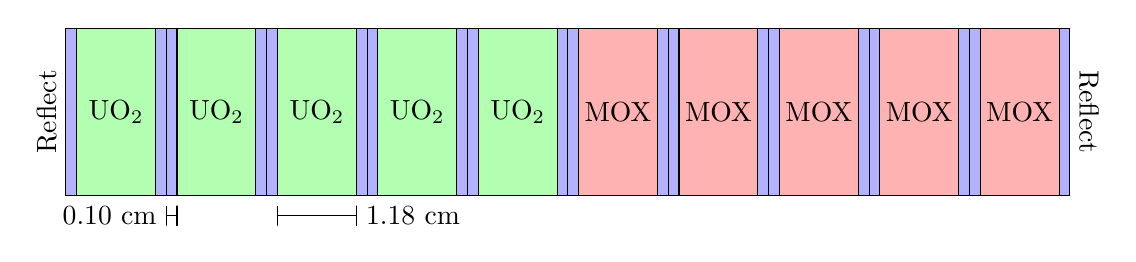
\begin{tikzpicture}[scale=0.85, every node/.style={scale=1}]
      \foreach \x in {0,1.5,...,6}
      \filldraw[xshift=\x cm, fill=green!30!white, draw=black] (0.160714286,0) rectangle (1.339285714,2.5) node[pos=.5] {UO$_2$};
      \foreach \x in {7.5,9,...,13.5}
      \filldraw[xshift=\x cm, fill=red!30!white, draw=black] (0.160714286,0) rectangle (1.339285714,2.5) node[pos=.5] {MOX};
      \foreach \x in {0,1.5,...,13.5}
      \filldraw[xshift=\x cm, fill=blue!30!white, draw=black] (0,0) rectangle (0.160714286,2.5);
      \foreach \x in {0,1.5,...,13.5}
      \filldraw[xshift=\x cm, fill=blue!30!white, draw=black] (1.339285714,0) rectangle (1.5,2.5);
      \draw[xshift=15cm,yshift=1.25cm] node[right] {\rotatebox{-90}{Reflect}};
      \draw[yshift=1.25cm] node[left] {\rotatebox{90}{Reflect}};
      \draw (1.5,-.15) -- (1.5,-.45) -- (1.5,-.30) node[left] {0.10 cm} -- (1.660714286,-.30) -- (1.660714286,-.15) -- (1.660714286, -.45);
      \draw (3.160714286,-.15) -- (3.160714286,-.45) -- (3.160714286,-.30) -- (4.339285714,-.30) node[right] {1.18 cm} -- (4.339285714,-.15) -- (4.339285714, -.45);
    \end{tikzpicture}
    \caption{Configuration for 10-pin Test Problem}
    \label{fig:10-pin_config}
  \end{figure*}
  
  Fuel pins were 1.08 cm thick with 0.09 cm of moderator on each side. The baseline pin cell discretization consisted
  of 22 mesh cells of fuel enclosed by three mesh cells of moderator on either side; therefore, each pin cell provided
  28 energy-dependent snapshots.
  
  The second test case, more indicative of a boiled water reactor (BWR), was comprised of 
  seven assemblies each with 10 pins.  Three core configurations were used, and each core configuration
  had two unique assemblies.  Three fuel types were used, including 4.5\% enriched UO$_2$, 2.5\% enriched UO$_2$,
  and 4.5\% enriched UO$_2$ with 5 wt\% Gd$_2$O$_3$.  Core and assembly configurations are shown in Fig. \ref{fig:BWRconfig}.
  Boundary conditions for this case were vacuum.
  
  \begin{figure*}[htb]
    \begin{minipage}[c]{\textwidth}
      \centering
      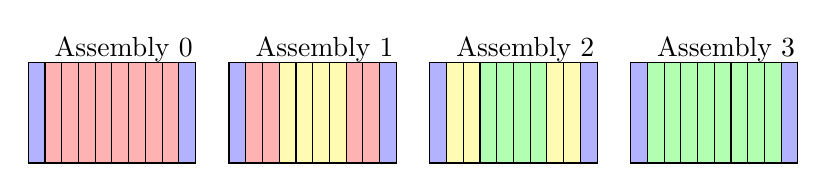
\begin{tikzpicture}[scale=0.85, every node/.style={scale=1}]
	\foreach \x in {0,2.25,3,5.25,6,8.25,9,11.25}
	\filldraw[xshift=\x cm,fill=blue!30!white,draw=black] (0,0) rectangle (0.25,1.5);
	\foreach \x in {.25,.5,.75,1,1.25,1.5,1.75,2,3.25,3.5,4.75,5}
	\filldraw[xshift=\x cm,fill=red!30!white,draw=black] (0,0) rectangle (0.25,1.5);
	\foreach \x in {3.75,4,4.25,4.5,6.25,6.5,7.75,8}
	\filldraw[xshift=\x cm,fill=yellow!30!white,draw=black] (0,0) rectangle (0.25,1.5);
	\foreach \x in {6.75,7,7.25,7.5,9.25,9.5,9.75,10,10.25,10.5,10.75,11}
	\filldraw[xshift=\x cm,fill=green!30!white,draw=black] (0,0) rectangle (0.25,1.5);
	\draw (0.25,1.7) node[right] {Assembly 0};%
	\draw (3.25,1.7) node[right] {Assembly 1};%
	\draw (6.25,1.7) node[right] {Assembly 2};%
	\draw (9.25,1.7) node[right] {Assembly 3};%
      \end{tikzpicture}
    \end{minipage} 
    \begin{minipage}[c]{\textwidth}
      \centering
      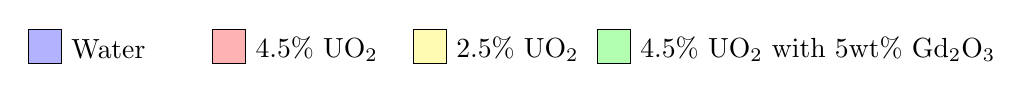
\begin{tikzpicture}[scale=0.85, every node/.style={scale=1}]
	\filldraw[xshift=-4cm,fill=blue!30!white,draw=black] (-.25,-.25) rectangle (.25,.25) node[yshift=-.25cm, right] {Water};%
	\filldraw[xshift=-1.25cm,fill=red!30!white,draw=black] (-.25,-.25) rectangle (.25,.25) node[yshift=-.25cm, right] {4.5$\%$ UO$_2$};%
	\filldraw[xshift=1.75cm,fill=yellow!30!white,draw=black] (-.25,-.25) rectangle (.25,.25) node[yshift=-.25cm, right] {2.5$\%$ UO$_2$};%
	\filldraw[xshift=4.5cm,fill=green!30!white,draw=black] (-.25,-.25) rectangle (.25,.25) node[yshift=-.25cm, right] {4.5$\%$ UO$_2$ with 5wt$\%$ Gd$_2$O$_3$};%
      \end{tikzpicture}
    \end{minipage}
    \begin{minipage}[c]{\textwidth}
      \centering
      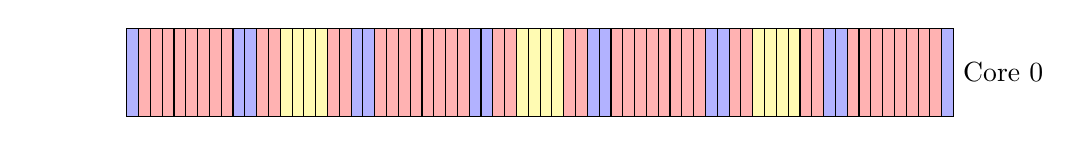
\begin{tikzpicture}[scale=1.5, every node/.style={scale=1}]
	\foreach \x in {0,.1,...,6.9}
	\filldraw[xshift=\x cm,fill=red!30!white,draw=black] (0,0) rectangle (0.1,.75);
	\foreach \x in {0,1,2,3,4,5,6,.9,1.9,2.9,3.9,4.9,5.9,6.9}
	\filldraw[xshift=\x cm,fill=blue!30!white,draw=black] (0,0) rectangle (0.1,.75);
	\foreach \x in {1.3,1.4,1.5,1.6,3.3,3.4,3.5,3.6,5.3,5.4,5.5,5.6}
	\filldraw[xshift=\x cm,fill=yellow!30!white,draw=black] (0,0) rectangle (0.1,.75);
	\draw (7,.375) node[right] {Core 0};%
	\draw (0,.375) node[left,color=white] {Core 0};
      \end{tikzpicture}
    \end{minipage}
    \begin{minipage}[c]{\textwidth}
      \centering
      \vspace*{.15cm}
      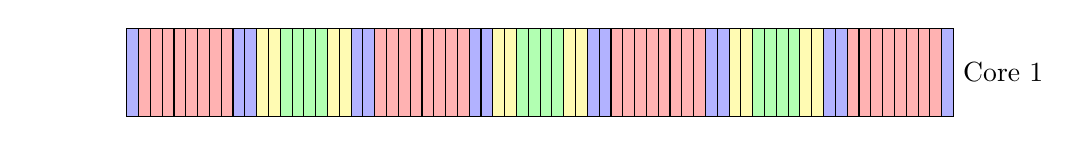
\begin{tikzpicture}[scale=1.5, every node/.style={scale=1}]
	\foreach \x in {0,.1,...,6.9}
	\filldraw[xshift=\x cm,fill=red!30!white,draw=black] (0,0) rectangle (0.1,.75);
	\foreach \x in {0,1,2,3,4,5,6,.9,1.9,2.9,3.9,4.9,5.9,6.9}
	\filldraw[xshift=\x cm,fill=blue!30!white,draw=black] (0,0) rectangle (0.1,.75);
	\foreach \x in {1.1,1.2,1.7,1.8,3.1,3.2,3.7,3.8,5.1,5.2,5.7,5.8}
	\filldraw[xshift=\x cm,fill=yellow!30!white,draw=black] (0,0) rectangle (0.1,.75);
	\foreach \x in {1.3,1.4,1.5,1.6,3.3,3.4,3.5,3.6,5.3,5.4,5.5,5.6}
	\filldraw[xshift=\x cm,fill=green!30!white,draw=black] (0,0) rectangle (0.1,.75);
	\draw (7,.375) node[right] {Core 1};%
	\draw (0,.375) node[left,color=white] {Core 1};
      \end{tikzpicture}
    \end{minipage}
    \begin{minipage}[c]{\textwidth}
      \centering
      \vspace*{.15cm}
      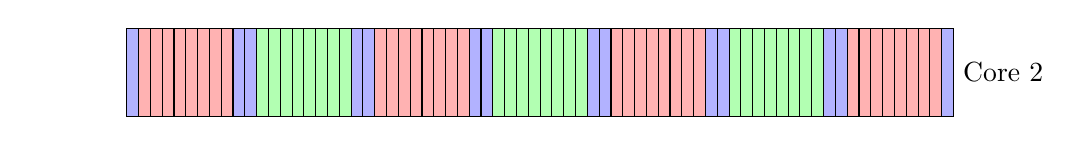
\begin{tikzpicture}[scale=1.5, every node/.style={scale=1}]
	\foreach \x in {0,.1,...,6.9}
	\filldraw[xshift=\x cm,fill=red!30!white,draw=black] (0,0) rectangle (0.1,.75);
	\foreach \x in {0,1,2,3,4,5,6,.9,1.9,2.9,3.9,4.9,5.9,6.9}
	\filldraw[xshift=\x cm,fill=blue!30!white,draw=black] (0,0) rectangle (0.1,.75);
	\foreach \x in {1.1,1.2,1.3,1.4,1.5,1.6,1.7,1.8,3.1,3.2,3.3,3.4,3.5,3.6,3.7,3.8,5.1,5.2,5.3,5.4,5.5,5.6,5.7,5.8}
	\filldraw[xshift=\x cm,fill=green!30!white,draw=black] (0,0) rectangle (0.1,.75);
	\draw (7,.375) node[right] {Core 2};%
	\draw (0,.375) node[left,color=white] {Core 2};
      \end{tikzpicture}
    \end{minipage}
    \caption{Configuration for BWR Test Problem}
    \label{fig:BWRconfig}
  \end{figure*}  
  
    Fuel pins for the second problem were 0.72 cm thick with 0.27 cm of 
    moderator on each side. Baseline pin cell discretization consisted of 16 
    mesh cells of fuel enclosed by six mesh cells of moderator; therefore, each 
    pin cell provided 28 energy-dependent snapshots. With 70 pin cells, the 
    total number of snapshots was 1960, but the right set of snapshots was 
    identical to the left with respect to scalar flux.
  
  Because the test problem reference solution is a full transport approximation, boundary currents generally
  exhibit coupled angle-energy dependence.  By including snapshots that incorporate angular information,
  resulting KLT basis may outperform snapshots based only on scalar flux, $\phi$.  To include angular information, 
  snapshots were taken of the energy-dependent partial current, $J_{\text{left}}$.  Snapshots of the net
  current were previously considered, but those snapshots preformed equal to or worse than the 
  partial current in all cases, so they are not presented here.  Direction for the partial current is arbitrary
  because the snapshot models were symmetric. Because step-characteristics discretization produces only one
  spatial unknown per cell, the snapshot generation approach used provided one ($\phi$) or two 
  ($\phi$ and $J_{\text{left}}$) snapshots per spatial cell.
  
  In addition to inclusion of snapshots of partial current for each test problem, the addition of snapshots of higher
  order angular moments were studied.  These moments were generated by expanding the angular flux, $\Psi$,  
  through a Jacobi expansion in angle.  By this method the $0^{th}$ moment is equivalent to the partial current,
  while higher moments have less defined physical corollaries.  Inclusion of these moments (up to $3^{rd}$ order)
  was studied for both test problems and results are presented at the end of the results section.
  
  \subsection{Generation of Snapshots for Test Problems}
  
  Ideally, with any form of model reduction, computational effort required to solve a given problem is reduced, so a 
  quickly computed basis set is sought. Therefore, the generation of snapshots for KLT was a primary focus for 
  this work.  
  
  The first test problem was a 1-D approximation of the junction between a UO$_2$ and MOX assembly.  
  Therefore, a number of small, representative subproblems are clear choices for snapshot generation.  
  Models studied for this problem are summarized in Table \ref{tab:snapshots}.
  The simplest approach for generating snapshots is to model each pincell individually, subject to 
  reflecting boundary conditions on all surfaces and to extract snapshots (i.e., energy-dependent vectors
  in distinct spatial cells) from an individual pincell or combine snapshots from both pincell models.  
  
  \begin{table*}[htb]
    \centering
    \caption{Summary of models used for snapshot generation for 10-pin test case}
    \begin{tabular}{c | l}\toprule
      Abbreviation    & Model to generate snapshots \\ \midrule
      MOX Pin         & MOX pin only \\
      UO$_2$ Pin      & UO$_2$ pin only \\
      Combined Pins   & Combined snapshots from UO$_2$ and MOX models, and two-pin, UO$_2$-MOX model \\
      Full Assembly   & Repeating array of 10 UO$_2$ and 10 MOX pins \\
      \bottomrule
    \end{tabular}
    \label{tab:snapshots}
  \end{table*}
  
  A larger energy space is obtained if a single model includes more than one pin (fuel or moderator) 
  in various arrangements.  For this work, an effectively $10\times 10$ (infinite lattice of ten UO$_2$ and ten MOX pins; 
  denoted as the full assembly) was studied.  The full assembly model
  is the test problem of interest and should be expected to yield snapshots that represent the true multigroup
  solution with the lowest-order energy expansion.  Although other configurations were studied, configurations chosen for presentation provide
  a view into KLT using realistically attainable snapshots compared to the test problem.
  
  The second test problem was a 1-D approximation for a BWR core.  Models for this case are summarized in 
  Table \ref{tab:bwrsnapshots}.  Three cases naturally arise from core construction: snapshots
  from the entire core which are expected to perform the best, snapshots from the two unique
  assemblies used for each core configuration, and snapshots from each unique fuel pin used in the
  core configuration.  
  
  \begin{table*}[htb]
    \centering
    \caption{Summary of models used for snapshot generation for BWR test case}
    \begin{tabular}{c | l}\toprule
      Abbreviation         & Model to generate snapshots \\ \midrule
      Full Core            & Snapshots from whole core model (i.e., the test problem) \\
      Combined Assemblies  & Snapshots from unique assemblies used in core configuration \\
      Combined Pins        & Snapshots from unique pins used in core configuration \\
      \bottomrule
    \end{tabular}
    \label{tab:bwrsnapshots}
  \end{table*}
  
  \section{Results and Discussion}
  
  Typically, reactor analysis attempts to compute pin fission densities 
  (or powers) with sub-$1\%$ errors.  To add an additional 
  buffer, the goal of this work is to minimize the energy expansion order 
  required to achieve sub-$0.1\%$ maximum relative fission density errors.
  The reference solution in all cases was a full multigroup response matrix solution for the given test problem
  with consistent angular expansion used throughout; in other words, any observed
  changes in the solution when using various energy bases was a 
  function of only the energy basis.
  
  With the exception of `DLP' and `mDLP', each curve was generated using KLT basis with distinct snapshot data.
  The mDLP results represent the best case previously observed in \REF{Roberts2014}, which was to modify DLP with
  the average flux profile from the complete model.  Therefore, mDLP results are not realistic because the solution
  for the test problem must be known {\it a priori}.
  
  Because the test problem and snapshot models studied were relatively small, timing studies would 
  provide little insight.  However, for large 2-D or 3-D models (e.g., assemblies or full cores), the snapshot
  models (e.g., pin cells or sub-assemblies) should be orders of magnitude less computationally expensive
  than the full model of interest.
  
  To improve computation time, databases that included responses for every order were created for each problem, 
  allowing the relevant information to be read quickly.  Responses are a function of the $k$ eigenvalue; thus, a study into
  the number of $k$ values and range of $k$ values was explored.  Responses varied weakly with $k$, thus databases with 8 $k$ values
  within a range of $\pm0.15$ of the solution eigenvalue were sufficient for the experiment.  This database size allowed
  for $3^{rd}$ order interpolation of responses.
  
  \subsection{10-pin Test Problem}
  
  As shown in Fig. \ref{fig:10pin-44}, almost all KLT bases outperformed DLP for nearly all orders in the 10-pin problem while using the 44-group library.  
  Snapshots generated by including UO$_2$ and MOX data perform as well as or better than mDLP, but single pin
  models did not perform as well as mDLP.  However, mDLP was calculated using the solution, whereas the single pin models did not.
  
  \begin{figure*}[!ht]
    \centering
    \begin{subfigure}{0.5\textwidth}
      \centering
      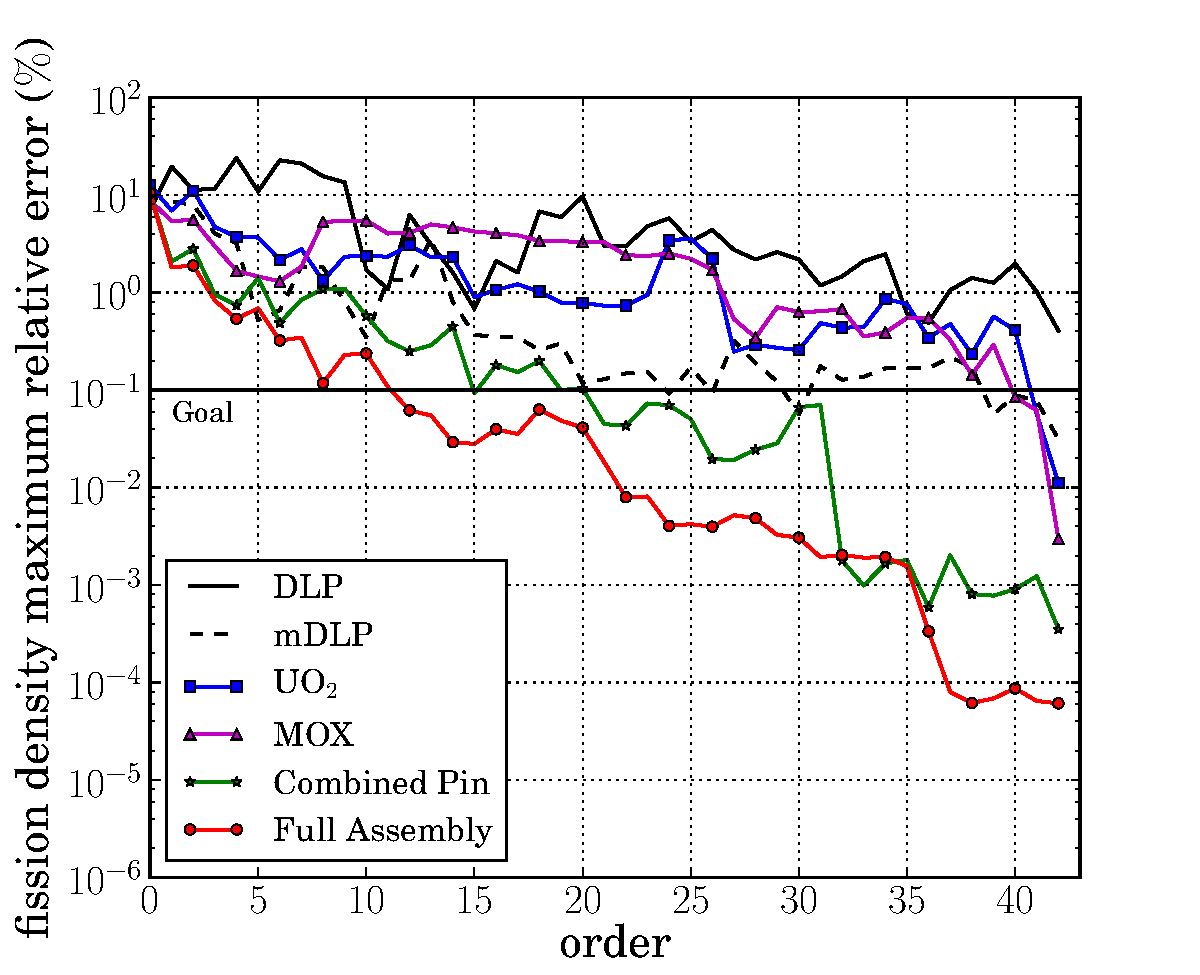
\includegraphics[trim=.1cm .25cm 2.0cm .4cm, clip=true, totalheight=0.28\textheight]{10pin_44_energy_basis_comparison_fission-44}
      \caption{Using only $\phi$ data}
      \label{fig:10pin-44a}
    \end{subfigure}%
    \begin{subfigure}{0.5\textwidth}
      \centering
      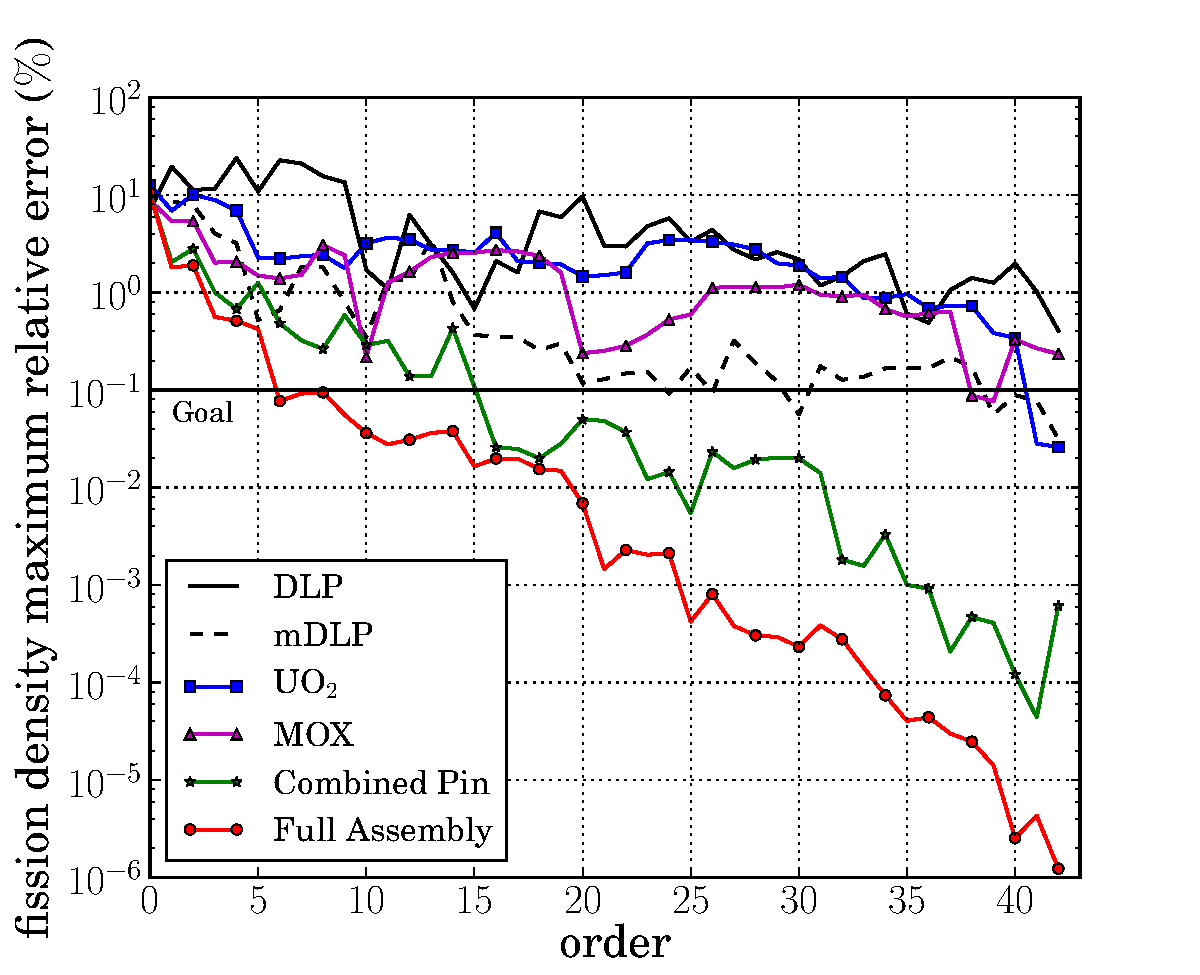
\includegraphics[trim=.1cm .25cm 2.0cm .4cm, clip=true, totalheight=0.28\textheight]{10pin_44_partial_energy_basis_comparison_fission-44}
      \caption{Using $\phi$ and $J_{\text{left}}$ data}
      \label{fig:10pin-44b}
    \end{subfigure}
    \caption{Relative error for 10-pin problem from 44-group library}
    \label{fig:10pin-44}
  \end{figure*}
  
  Fig. \ref{fig:10pin-44a} shows results of using only scalar flux, $\phi$, as data for snapshots.  When using snapshots
  from the full assembly model, relative error fell below the 0.1$\%$ threshold at an energy
  order of approximately 12.  The combined pin model required an energy expansion order of at least 20, far from the goal of approximately five orders.
  
  When partial current snapshots were included with scalar flux, results were improved, as shown in Fig. \ref{fig:10pin-44b}.
  The full assembly snapshot model yielded sub-0.1$\%$ fission density errors with sixth order expansions.  The combined pin model required
  an energy expansion order of approximately 15.
  
  Results for the 238-group library were expected to be similar to the 44-group results.  Figures presented from the 238-group library
  are shown only to 43rd energy order to ease comparison to the 44-group library.  With respect to the goal of order reduction, models should
  reach the 0.1$\%$ threshold by energy order of 44 regardless.
  
  Fig. \ref{fig:10pin-238a} shows results of using only scalar flux, $\phi$, as data for snapshots.  When using snapshots 
  from the full assembly model, relative error fell below the 0.1$\%$ threshold at an energy order of approximately 14.
  The combined pin model required an energy expansion order of at least 25.  Low-order
  results from the 238-group library were similar to the 44-group results, specifically for KLT basis models.
  
  \begin{figure*}[!ht]
    \centering
    \begin{subfigure}{0.5\textwidth}
      \centering
      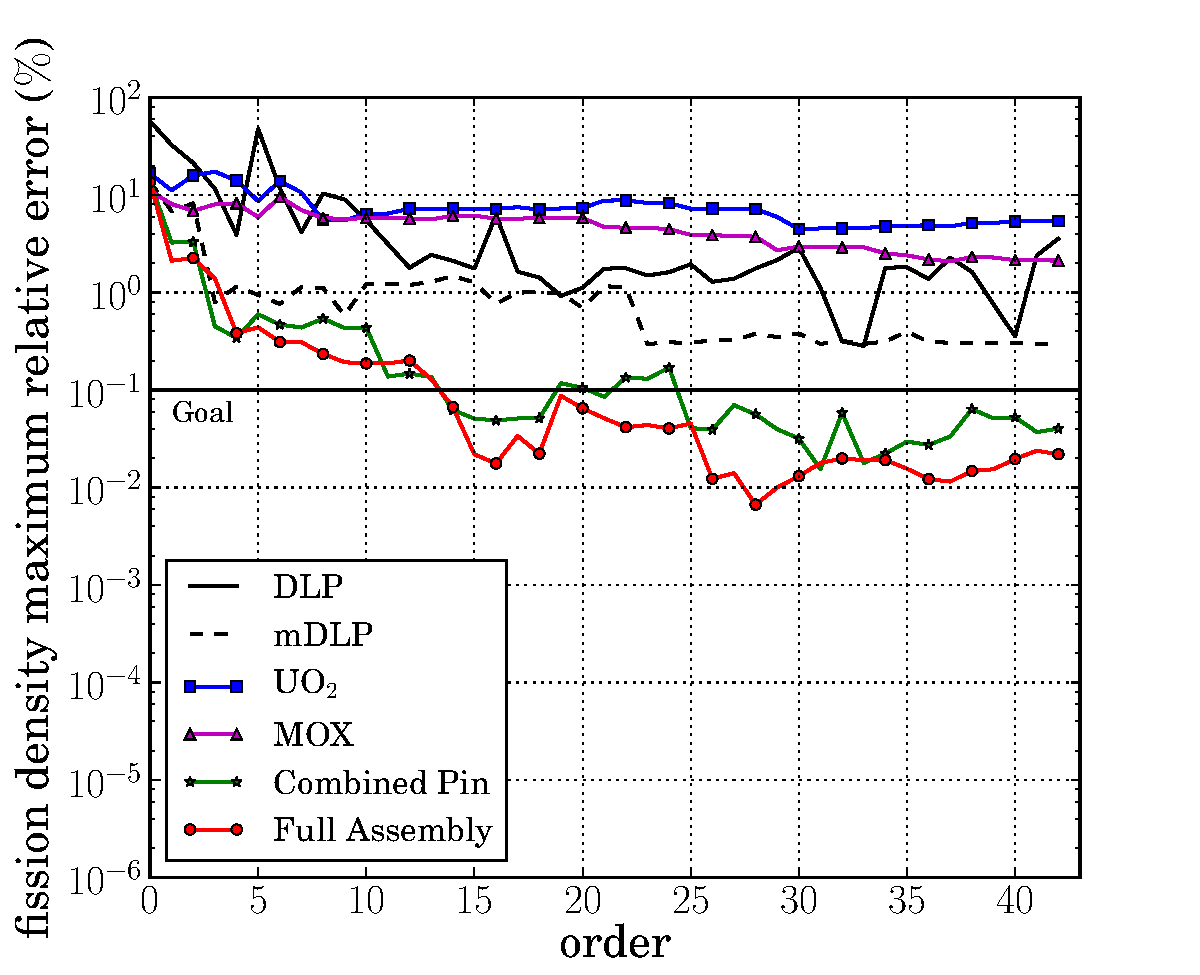
\includegraphics[trim=.1cm .25cm 2.0cm .4cm, clip=true, totalheight=0.28\textheight]{10pin_238_energy_basis_comparison_fission-44}
      \caption{Using only $\phi$ data}
      \label{fig:10pin-238a}
    \end{subfigure}%
    \begin{subfigure}{0.5\textwidth}
      \centering
      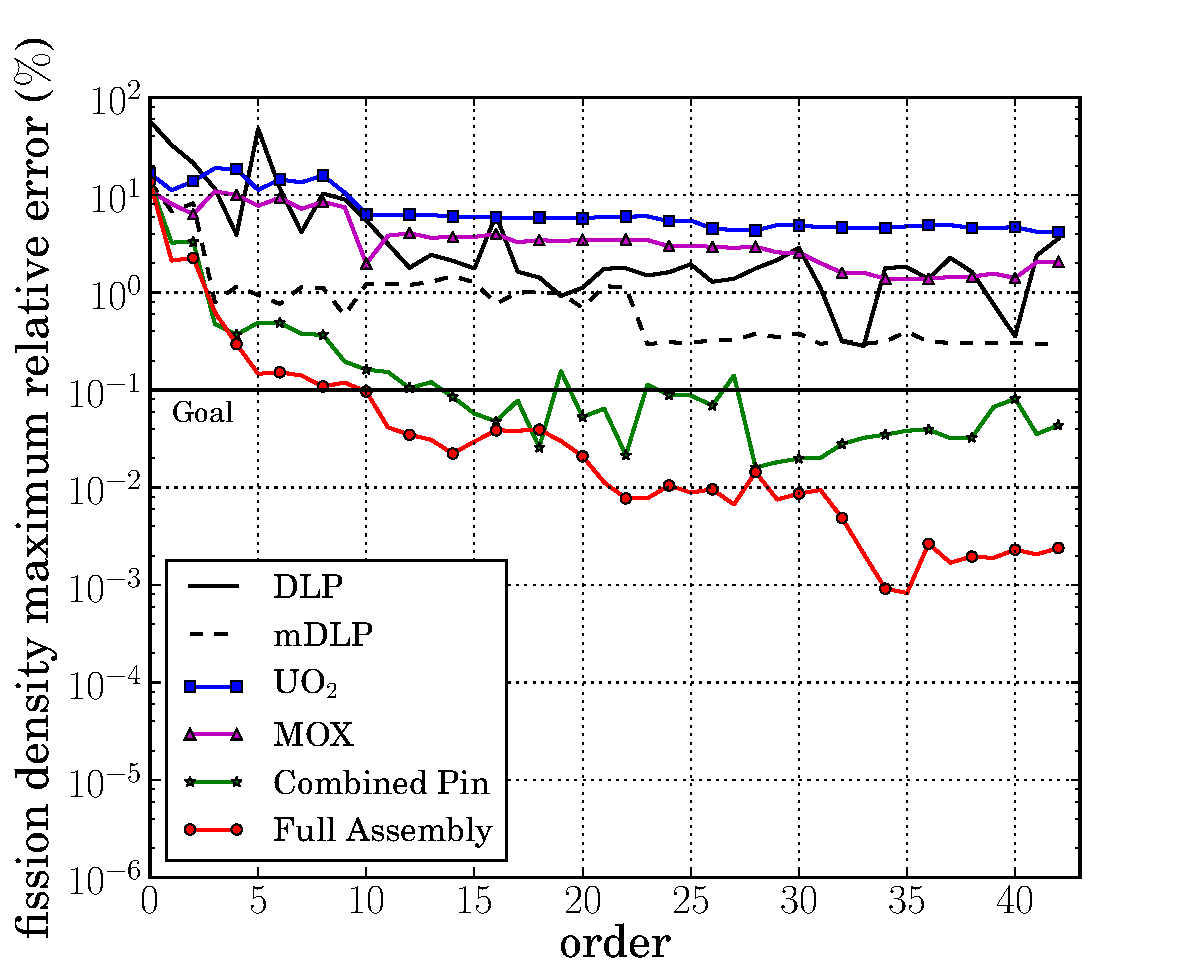
\includegraphics[trim=.1cm .25cm 2.0cm .4cm, clip=true, totalheight=0.28\textheight]{10pin_238_partial_energy_basis_comparison_fission-44}
      \caption{Using $\phi$ and $J_{\text{left}}$ data}
      \label{fig:10pin-238b}
    \end{subfigure}
    \caption{Relative error for 10-pin problem from 238-group library}
    \label{fig:10pin-238}
  \end{figure*}
  
  After snapshots from partial current were added to scalar flux snapshots, results of which are presented in Fig.\ref{fig:10pin-238b}.
  Inclusion of current snapshots improved the performance of each KLT model.  In the best case (full assembly model), the relative error dropped below 
  the 0.1$\%$ threshold at 10th order in energy, which was slightly improved from the 44-group results. The realistic model (combined pins) reaches the goal at
  an energy order of approximately 23.  
  
  In 44-group and 238-group library tests, the combined pin model preformed reasonably well compared to the full assembly model.  The combined pin
  model provided the realistic option for expanding in energy.  The full assembly model required the solution {\it a priori}, while the combined pins case utilized
  small problems to provide snapshots.  The single pin models, UO$_2$ and MOX, did not perform well, because the models
  lacked physics information for one of the fuel types.
  
  Inclusion of snapshots of higher-order angular moments for the 10-pin test problem are shown in Fig. \ref{fig:10-pin_angular}.  The curves
  were created using snapshots from the full assembly model.  Results from the 44-group and 238-group libraries are shown side-by-side to ease
  comparison.  The $0^{th}$ moment was equivalent to the leftward partial
  current, but the higher moments did not have direct physical corollaries.  Adding the higher moments did not significantly affect the 
  10-pin problem, consequently demonstrating that the relevant phase space information had already been captured. Therefore, curves for the higher moments
  were nearly equal to the $0^{th}$ moment curve.
  
  \begin{figure*}[!ht]
    \centering
    \begin{subfigure}{0.5\textwidth}
      \centering
      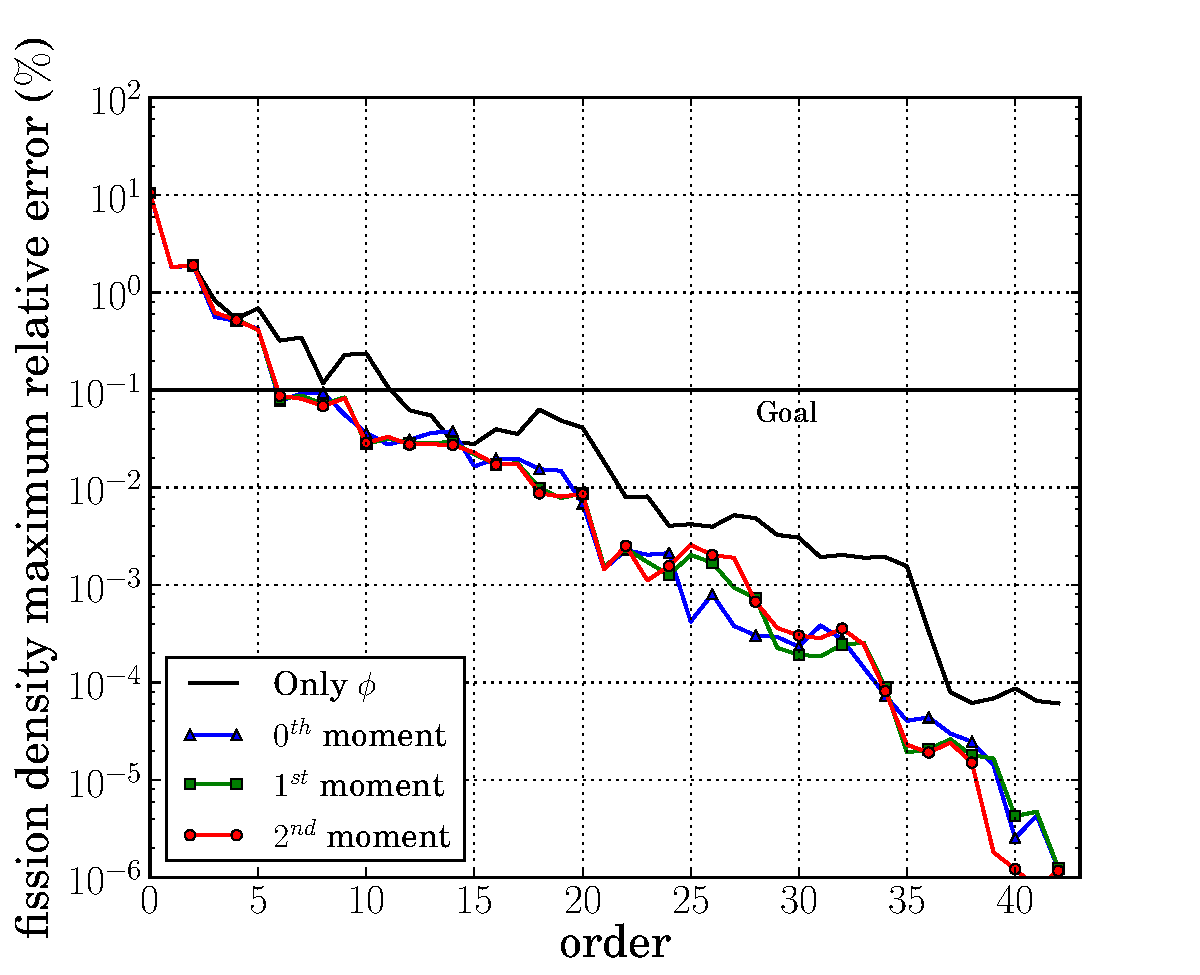
\includegraphics[trim=.1cm .25cm 2.0cm .4cm, clip=true, totalheight=0.28\textheight]{10pin_44_angular_comparison_fission_10-pin-44}
      \caption{From 44-group library}
      \label{fig:10-pin_angularA}
    \end{subfigure}%
    \begin{subfigure}{0.5\textwidth}
      \centering
      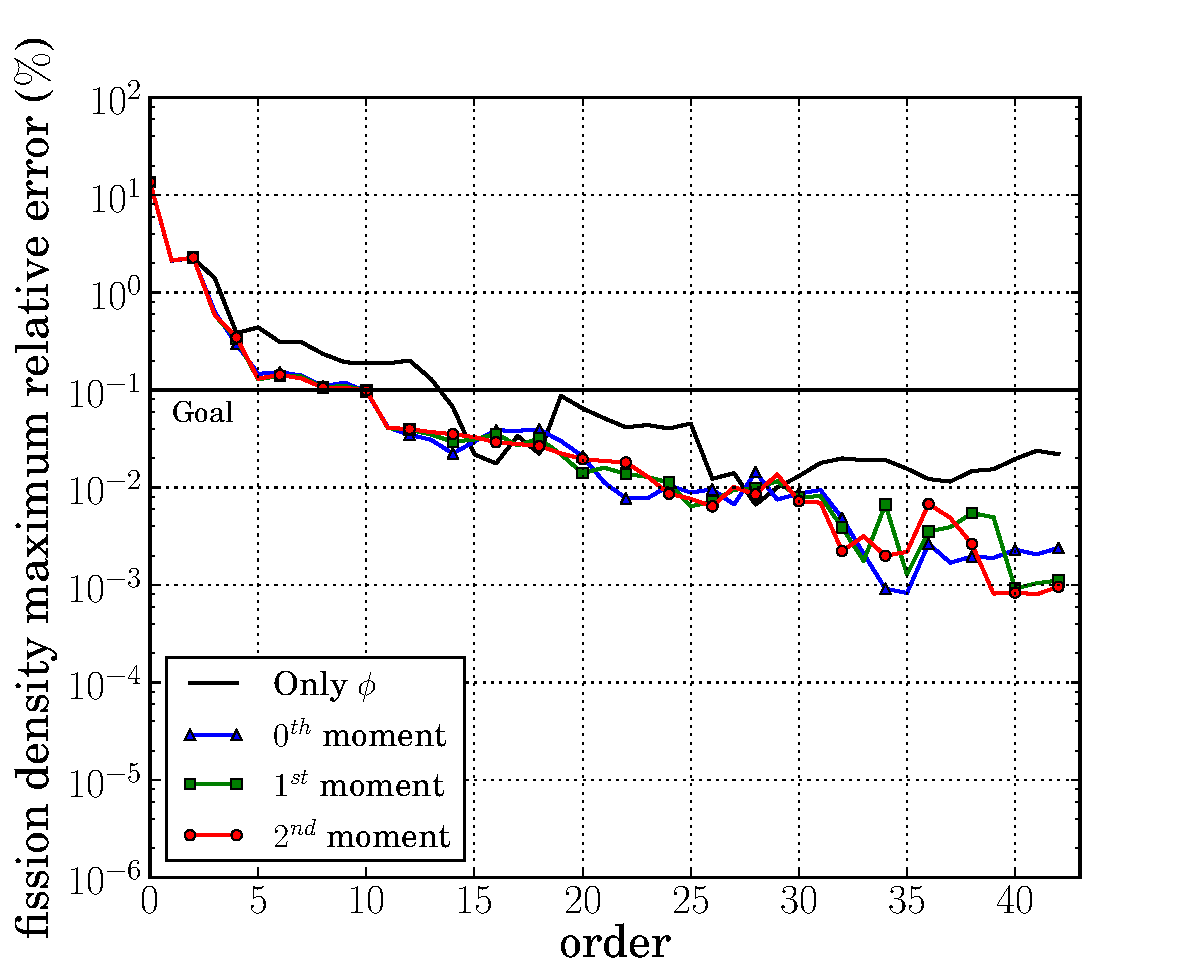
\includegraphics[trim=.1cm .25cm 2.0cm .4cm, clip=true, totalheight=0.28\textheight]{10pin_238_angular_comparison_fission_10-pin-44}
      \caption{From 238-group library}
      \label{fig:10-pin_angularB}
    \end{subfigure}
    \caption{Relative error for 10-pin problem using higher-order moment data}
    \label{fig:10-pin_angular}
  \end{figure*}
  
  \subsection{BWR Test Problem}
  
  For the BWR test problem, each core configuration was increasingly inhomogeneous, and thus, was more difficult.  The difficulty 
  manifests in a larger error for the same energy order while progressing through configurations.  In this section, described methods
  described were applied to the BWR test problem. The same goal of pin fission densities (or powers) with
  sub-$0.1\%$ maximum relative fission density errors was applied in this section.  The reference solution in all cases was a full multigroup response matrix
  solution of the BWR test problem; therefore, any observed changes in the solution when using various energy bases was a function of only the
  energy basis alone.  Results for the BWR problem were generated from a 44-group and a 238-group library as specified.
  
  Figures for this section are shown as side-by-side comparisons of using snapshots of only $\phi$ versus using snapshots
  including $\phi$ and the leftward partial current.  Three core configurations were explored, as shown.
  For the best case (using snapshots from the core model), Configuration 0, shown in 
  Fig. \ref{fig:core0-44}, took approximately six orders when
  using only scalar flux, and approximately five orders when including partial current.  Configuration 1, shown in Fig. \ref{fig:core1-44},
  required seven and eight orders, respectively, for using only $\phi$ and including partial current.  Finally, Configuration 2, shown in Fig. \ref{fig:core2-44},
  required 13 and 11 orders, respectively, to achieve the goal of sub-$0.1\%$ maximum relative fission density errors.  
  
  \begin{figure*}[!ht]
    \centering
    \begin{subfigure}{0.5\textwidth}
      \centering
      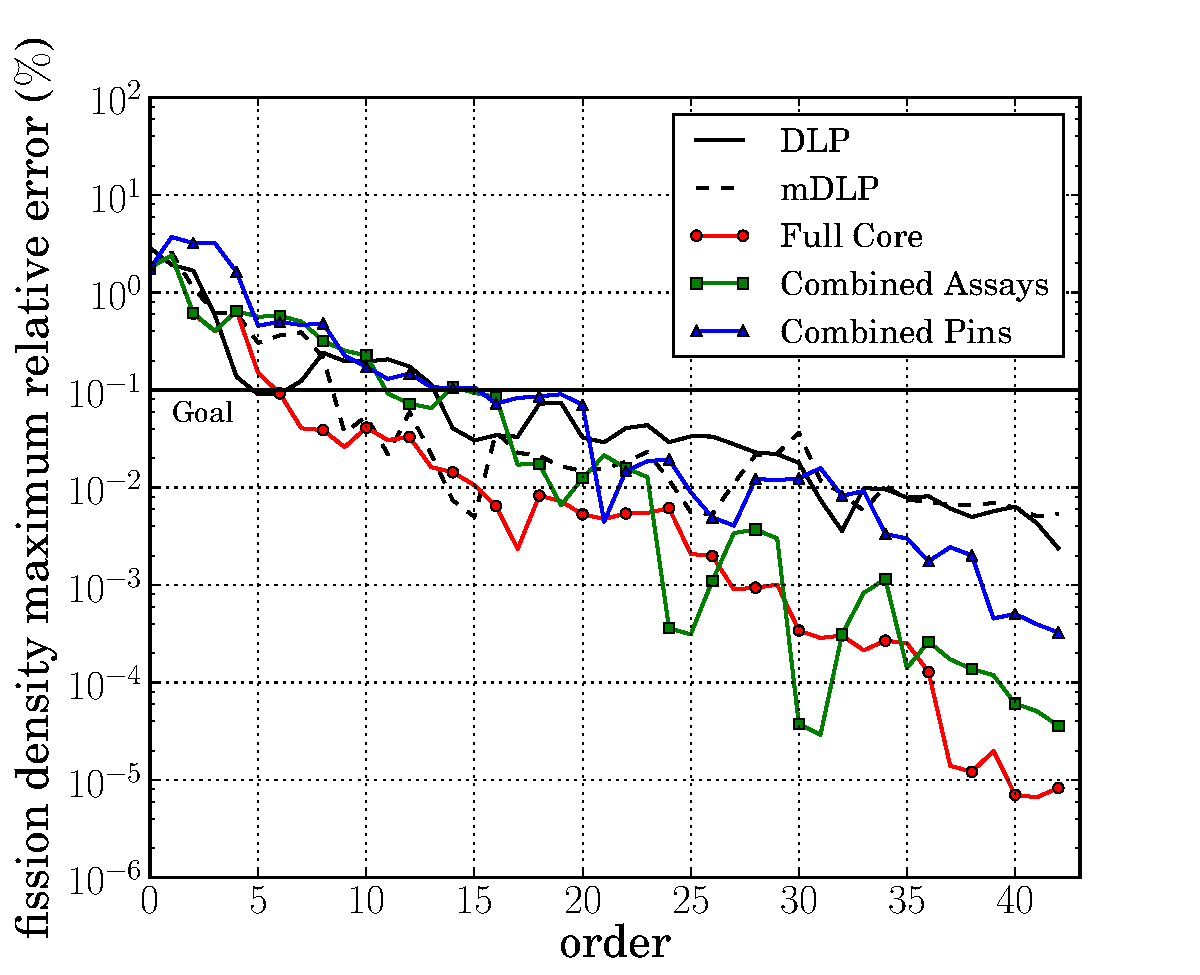
\includegraphics[trim=.1cm .25cm 2.0cm .4cm, clip=true, totalheight=0.28\textheight]{BWR0_44_energy_basis_comparison_fission-44}
      \caption{Using only $\phi$ data}
      \label{fig:core0-44a}
    \end{subfigure}%
    \begin{subfigure}{0.5\textwidth}
      \centering
      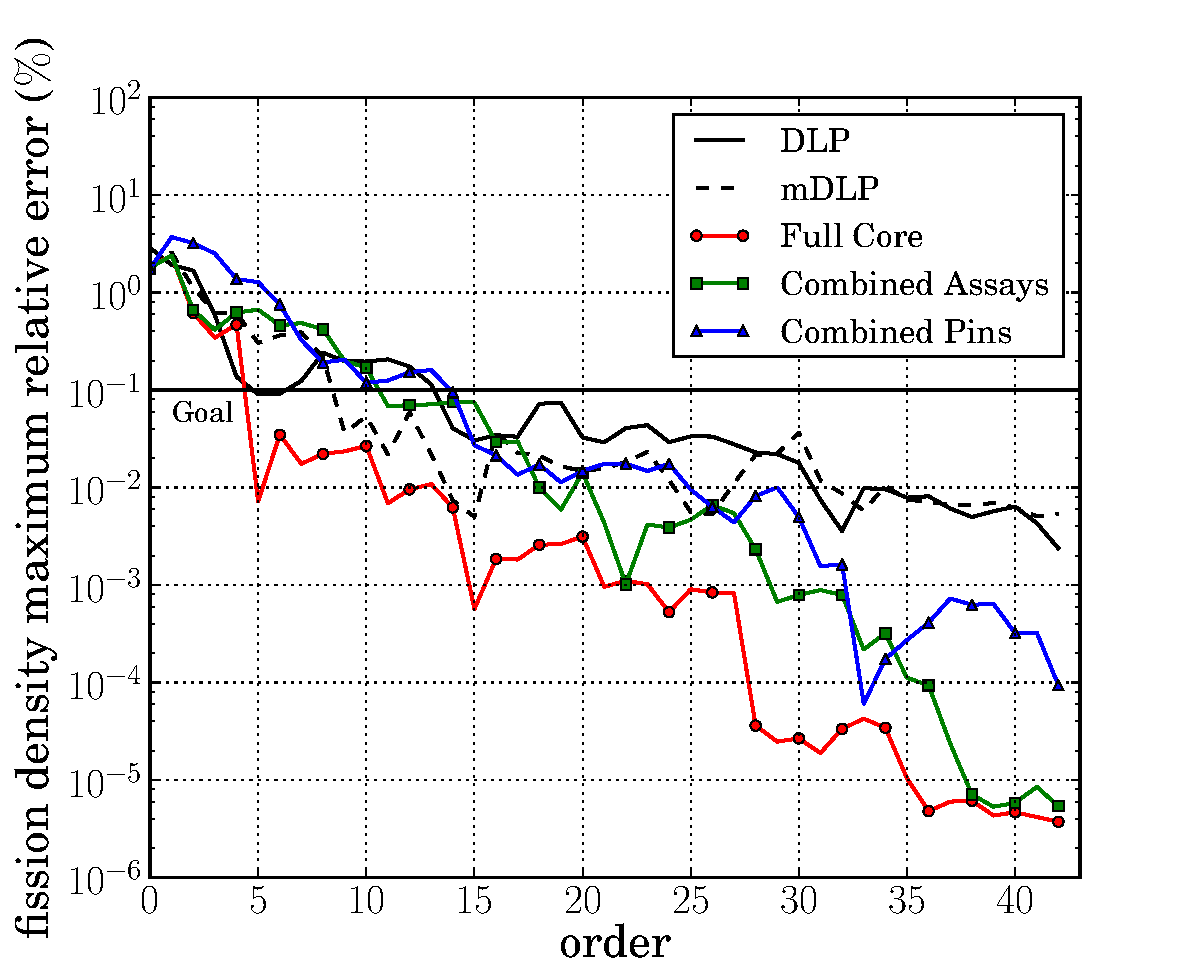
\includegraphics[trim=.1cm .25cm 2.0cm .4cm, clip=true, totalheight=0.28\textheight]{BWR0_44_partial_energy_basis_comparison_fission-44}
      \captionof{figure}{Using $\phi$ and $J_{\text{left}}$ data}
      \label{fig:core0-44b} 
    \end{subfigure}
    \caption{Relative error for BWR test problem, Configuration 0, from 44-group library}
    \label{fig:core0-44}
  \end{figure*}
  
  \begin{figure*}[!ht]
    \centering
    \begin{subfigure}{0.5\textwidth}
      \centering
      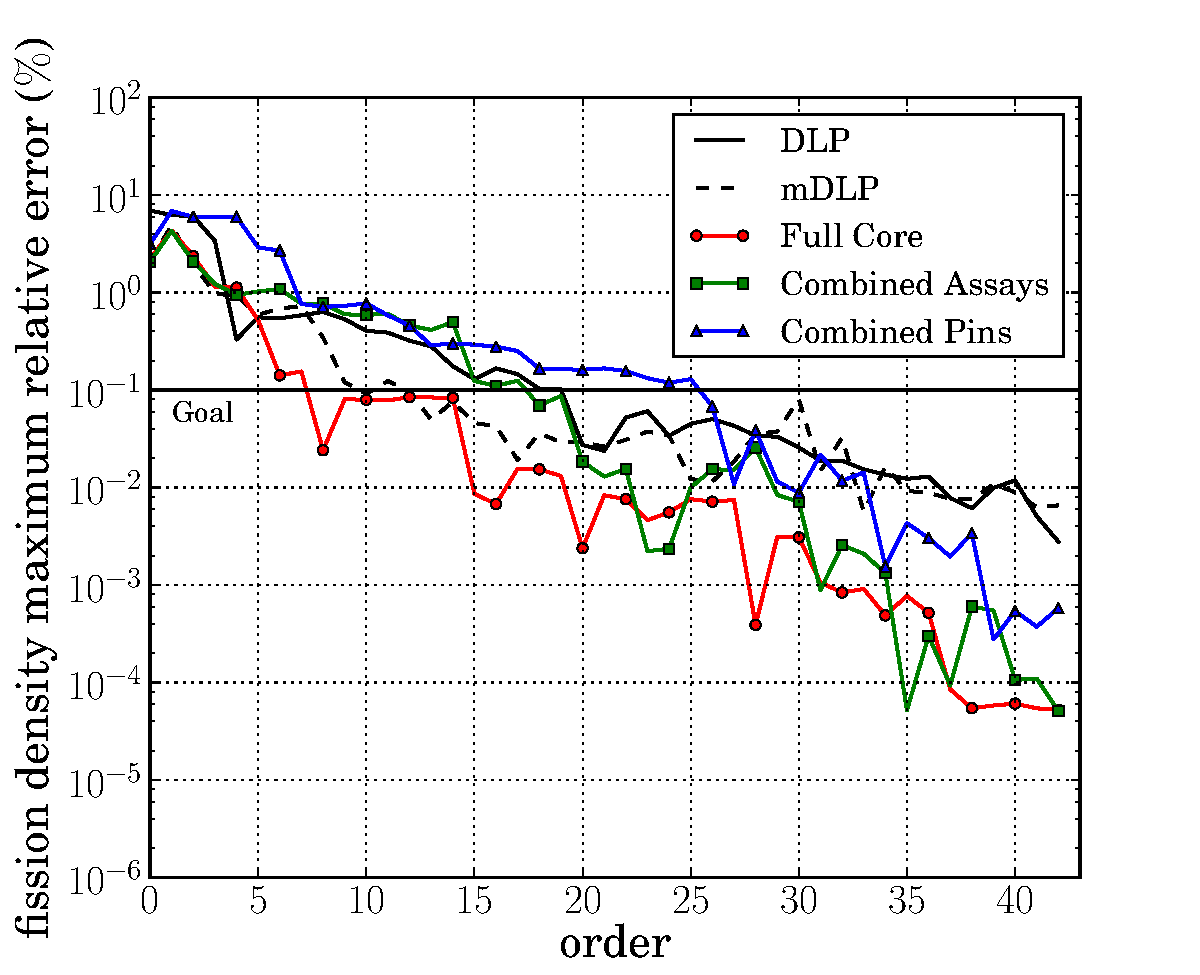
\includegraphics[trim=.1cm .25cm 2.0cm .4cm, clip=true, totalheight=0.28\textheight]{BWR1_44_energy_basis_comparison_fission-44}
      \caption{Using only $\phi$ data}
      \label{fig:core1-44a}
    \end{subfigure}%
    \begin{subfigure}{0.5\textwidth}
      \centering
      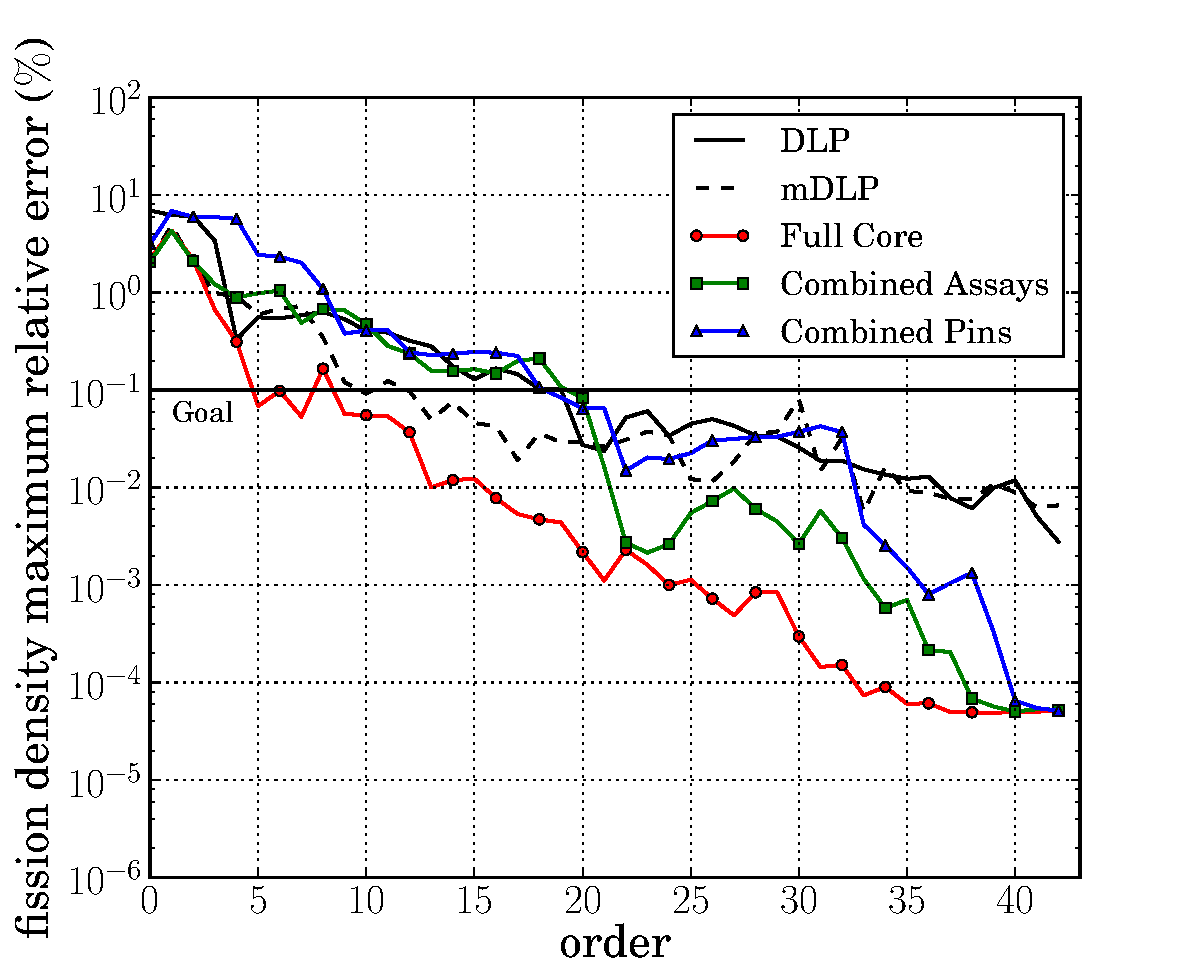
\includegraphics[trim=.1cm .25cm 2.0cm .4cm, clip=true, totalheight=0.28\textheight]{BWR1_44_partial_energy_basis_comparison_fission-44}
      \captionof{figure}{Using $\phi$ and $J_{\text{left}}$ data}
      \label{fig:core1-44b} 
    \end{subfigure}
    \caption{Relative error for BWR test problem, Configuration 1, from 44-group library}
    \label{fig:core1-44}
  \end{figure*}
  
  \begin{figure*}[!ht]
    \centering
    \begin{subfigure}{0.5\textwidth}
      \centering
      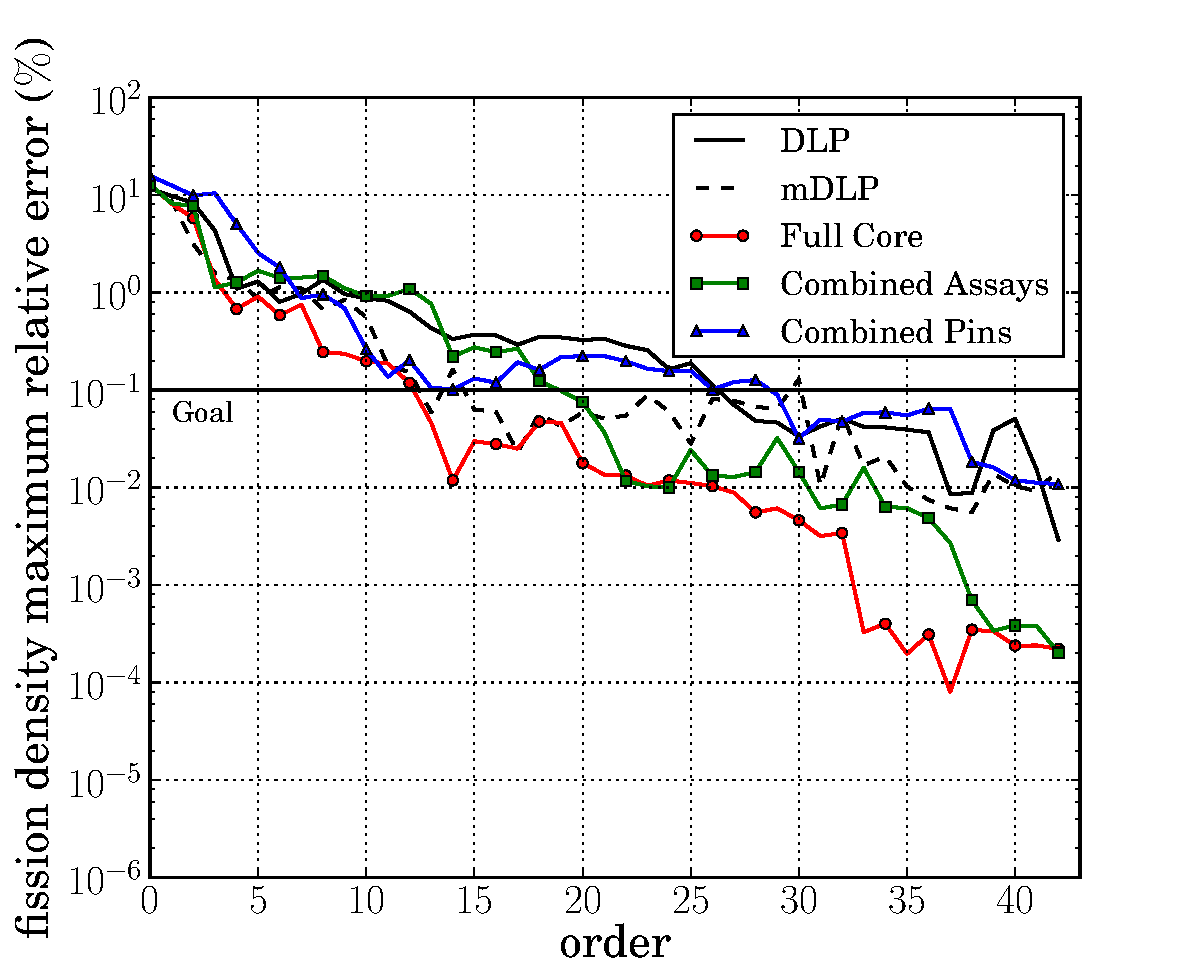
\includegraphics[trim=.1cm .25cm 2.0cm .4cm, clip=true, totalheight=0.28\textheight]{BWR2_44_energy_basis_comparison_fission-44}
      \caption{Using only $\phi$ data}
      \label{fig:core2-44a}
    \end{subfigure}%
    \begin{subfigure}{0.5\textwidth}
      \centering
      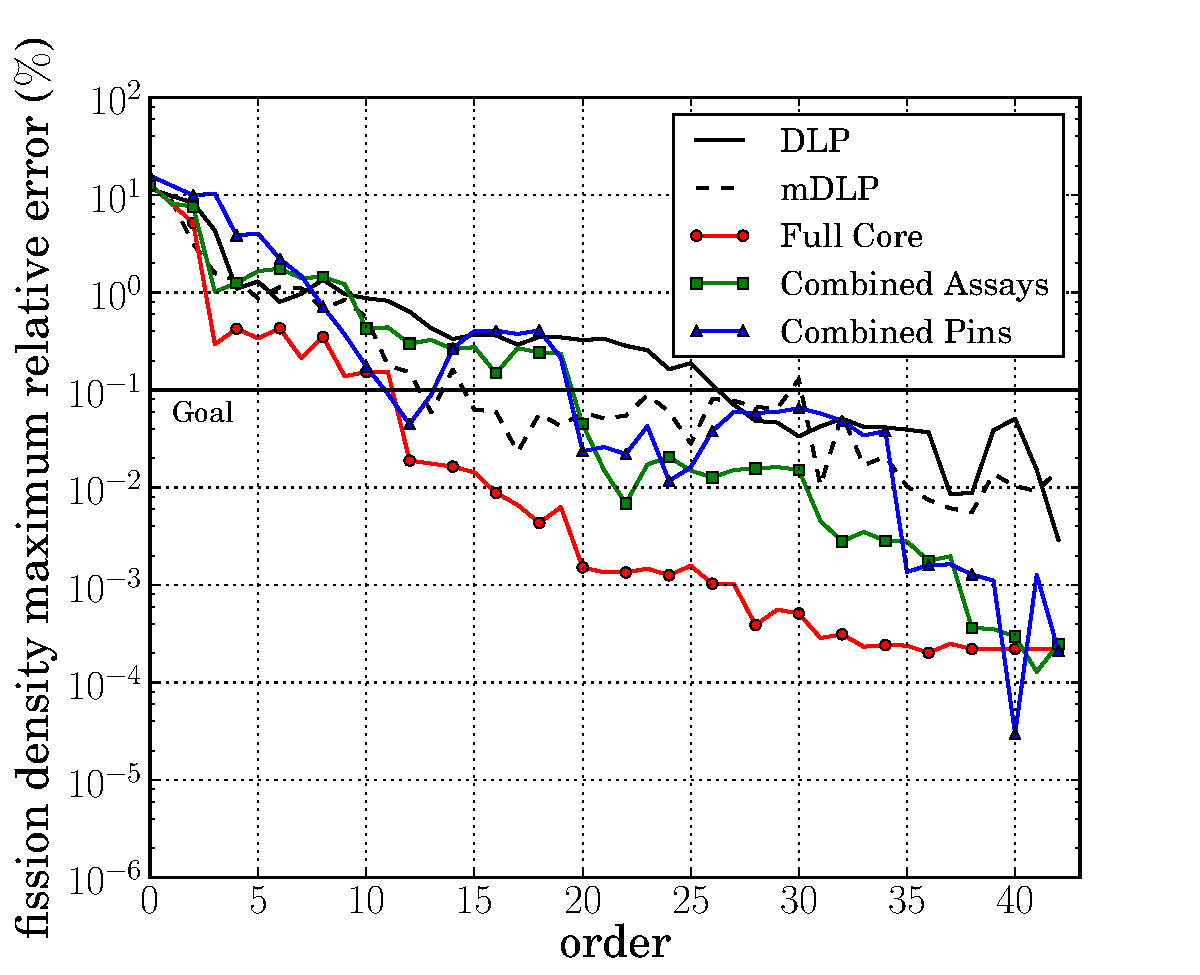
\includegraphics[trim=.1cm .25cm 2.0cm .4cm, clip=true, totalheight=0.28\textheight]{BWR2_44_partial_energy_basis_comparison_fission-44}
      \captionof{figure}{Using $\phi$ and $J_{\text{left}}$ data}
      \label{fig:core2-44b} 
    \end{subfigure}
    \caption{Relative error for BWR test problem, Configuration 2, from 44-group library}
    \label{fig:core2-44}
  \end{figure*}
  
  The realistic models, combined pins and combined assemblies, required energy order of approximately 15 and 14 when using only 
  scalar flux snapshot and using both scalar flux and partial current, respectively, for Configuration 0.  In Configuration 1,
  realistic models required at least order 20 to reach the goal while using only scalar flux.  Including partial current
  improved the results to 19th order.  Finally, Configuration 2 required approximately equivalent orders as Configuration 1 for realistic models
  
  The only configuration that met the second goal of an order of magnitude reduction in required energy order was the easiest configuration, 0.
  For the BWR test problem, the case of mDLP preformed much better as compared to the 10-pin test problem.
  However, mDLP uses the full core solution to generate modified polynomials, thus represented the best case for mDLP, but is not a realistic performance of mDLP.  
  For each core configuration, the combined pins and combined assemblies models performed similarly, but the combined assemblies model was superior.
  However, the performance of the combined pins model was gratifying due to the simplicity of the snapshot model.
  
  Analysis for the BWR test problem was repeated with a 238-group library.  In this case, Configuration 0, shown in Fig. \ref{fig:core0-238},
  required orders of 11 and 4, respectively, for only $\phi$ and including partial current.  Configuration 1, shown in Fig. \ref{fig:core1-238},
  requires orders of 12 and 9, respectively.  Configuration 2, shown in Fig. \ref{fig:core2-238}, required 22 and 10, respectively, 
  to meet the first goal of sub $0.1\%$ errors in fission density.
  
  \begin{figure*}[!ht]
    \centering
    \begin{subfigure}{0.5\textwidth}
      \centering
      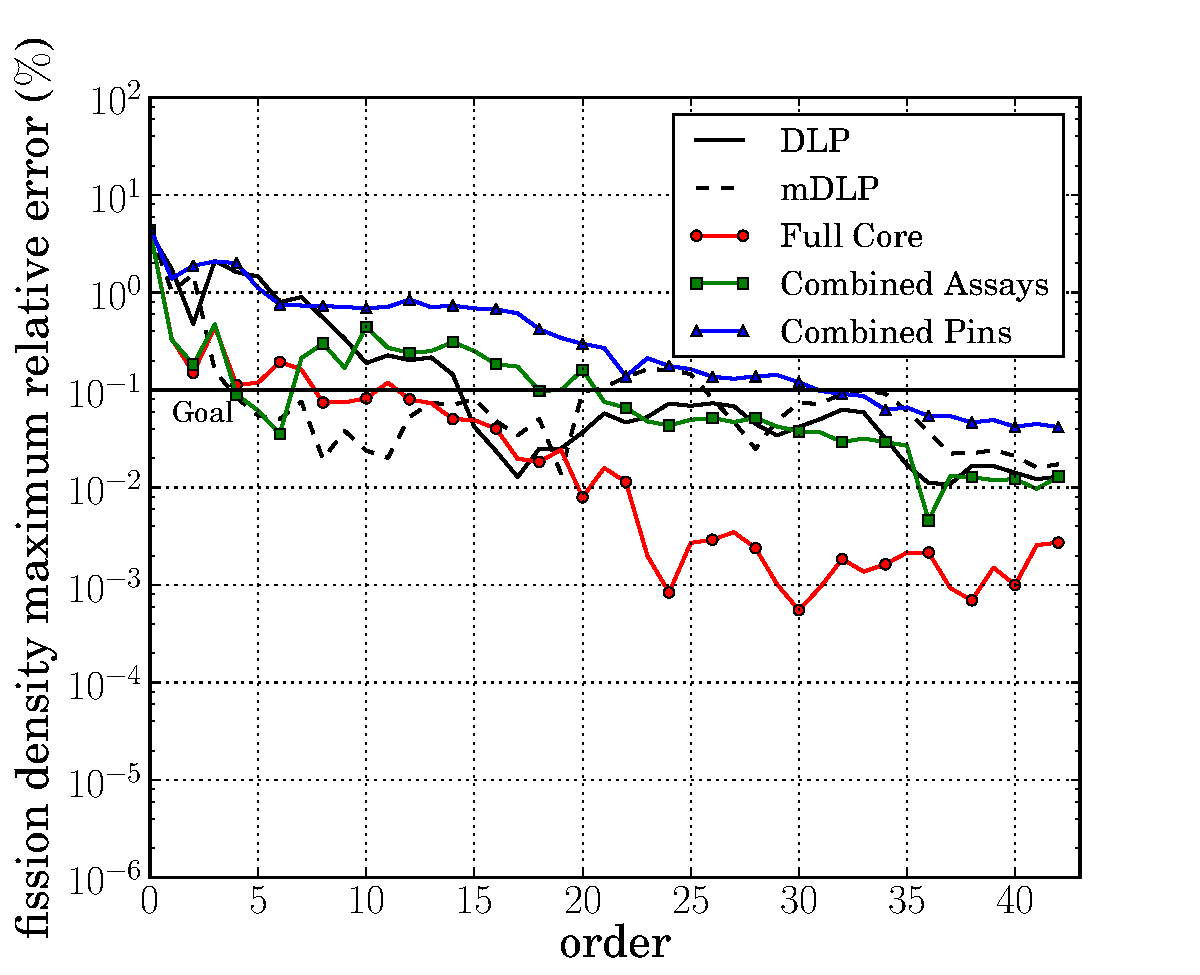
\includegraphics[trim=.1cm .25cm 2.0cm .4cm, clip=true, totalheight=0.28\textheight]{BWR0_238_energy_basis_comparison_fission-44}
      \caption{Using only $\phi$ data}
      \label{fig:core0-238a}
    \end{subfigure}%
    \begin{subfigure}{0.5\textwidth}
      \centering
      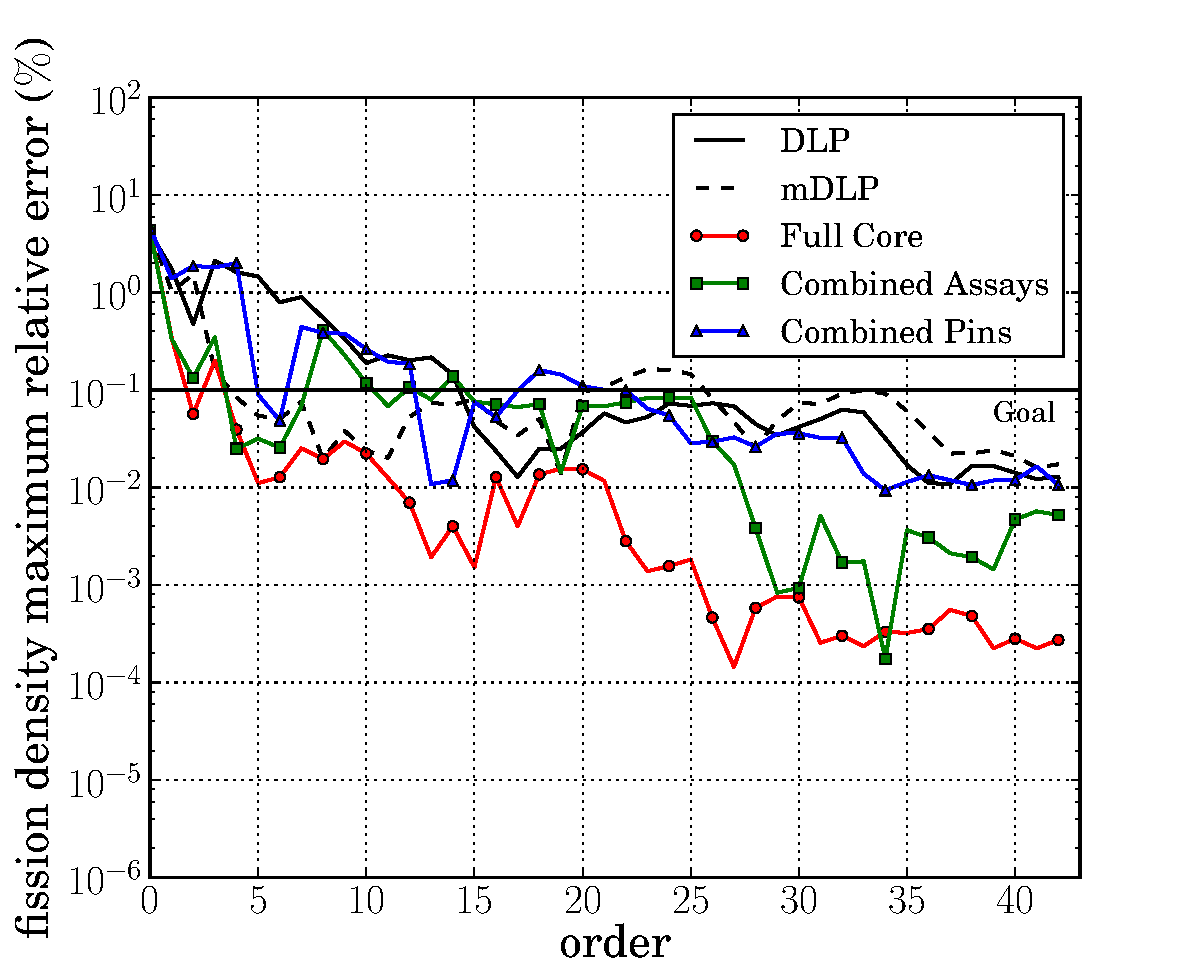
\includegraphics[trim=.1cm .25cm 2.0cm .4cm, clip=true, totalheight=0.28\textheight]{BWR0_238_partial_energy_basis_comparison_fission-44}
      \captionof{figure}{Using $\phi$ and $J_{\text{left}}$ data}
      \label{fig:core0-238b} 
    \end{subfigure}
    \caption{Relative error for BWR test problem, Configuration 0, from 238-group library}
    \label{fig:core0-238}
  \end{figure*}
  
  \begin{figure*}[!ht]
    \centering
    \begin{subfigure}{0.5\textwidth}
      \centering
      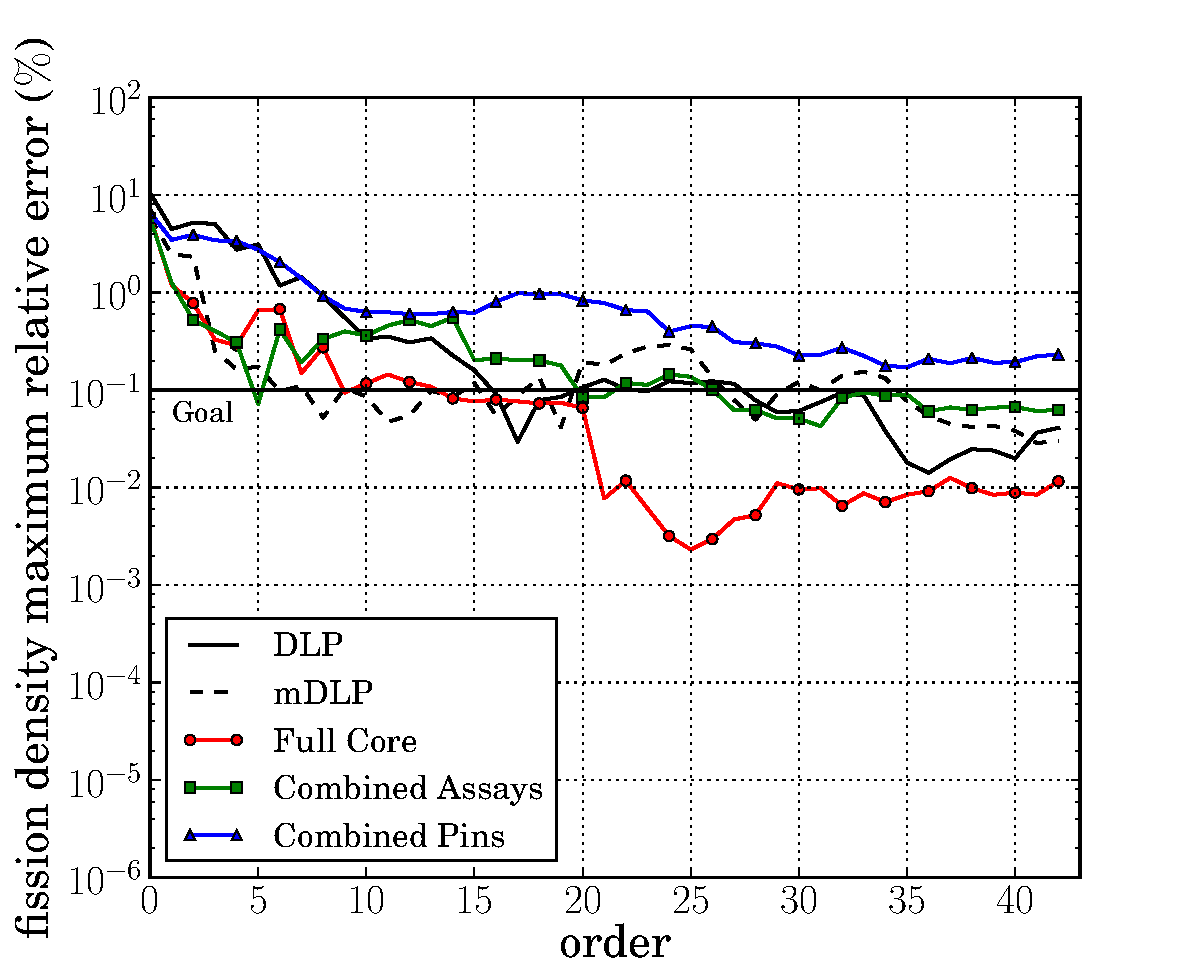
\includegraphics[trim=.1cm .25cm 2.0cm .4cm, clip=true, totalheight=0.28\textheight]{BWR1_238_energy_basis_comparison_fission-44}
      \caption{Using only $\phi$ data}
      \label{fig:core1-238a}
    \end{subfigure}%
    \begin{subfigure}{0.5\textwidth}
      \centering
      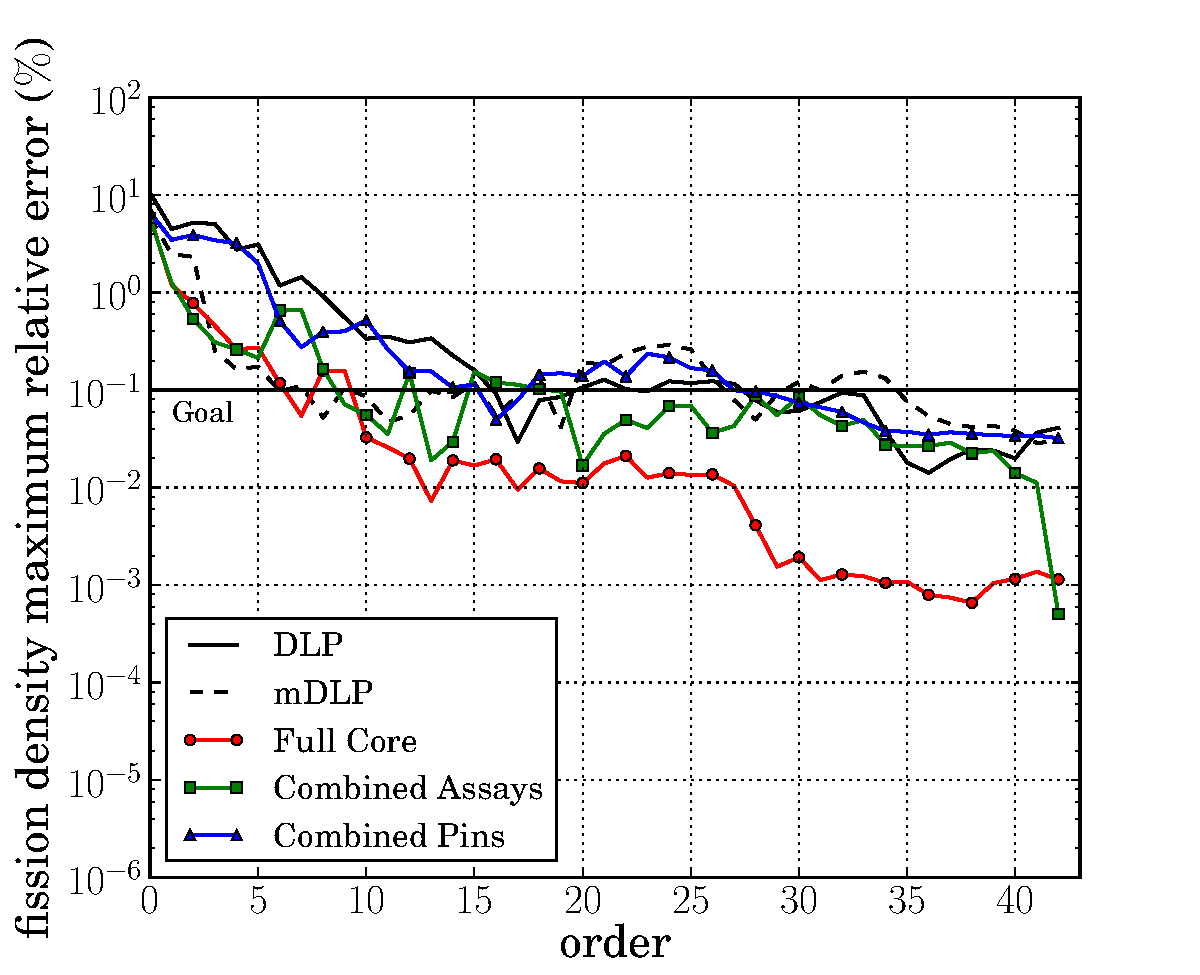
\includegraphics[trim=.1cm .25cm 2.0cm .4cm, clip=true, totalheight=0.28\textheight]{BWR1_238_partial_energy_basis_comparison_fission-44}
      \captionof{figure}{Using $\phi$ and $J_{\text{left}}$ data}
      \label{fig:core1-238b} 
    \end{subfigure}
    \caption{Relative error for BWR test problem, Configuration 1, from 238-group library}
    \label{fig:core1-238}
  \end{figure*}
  
  \begin{figure*}[!ht]
    \centering
    \begin{subfigure}{0.5\textwidth}
      \centering
      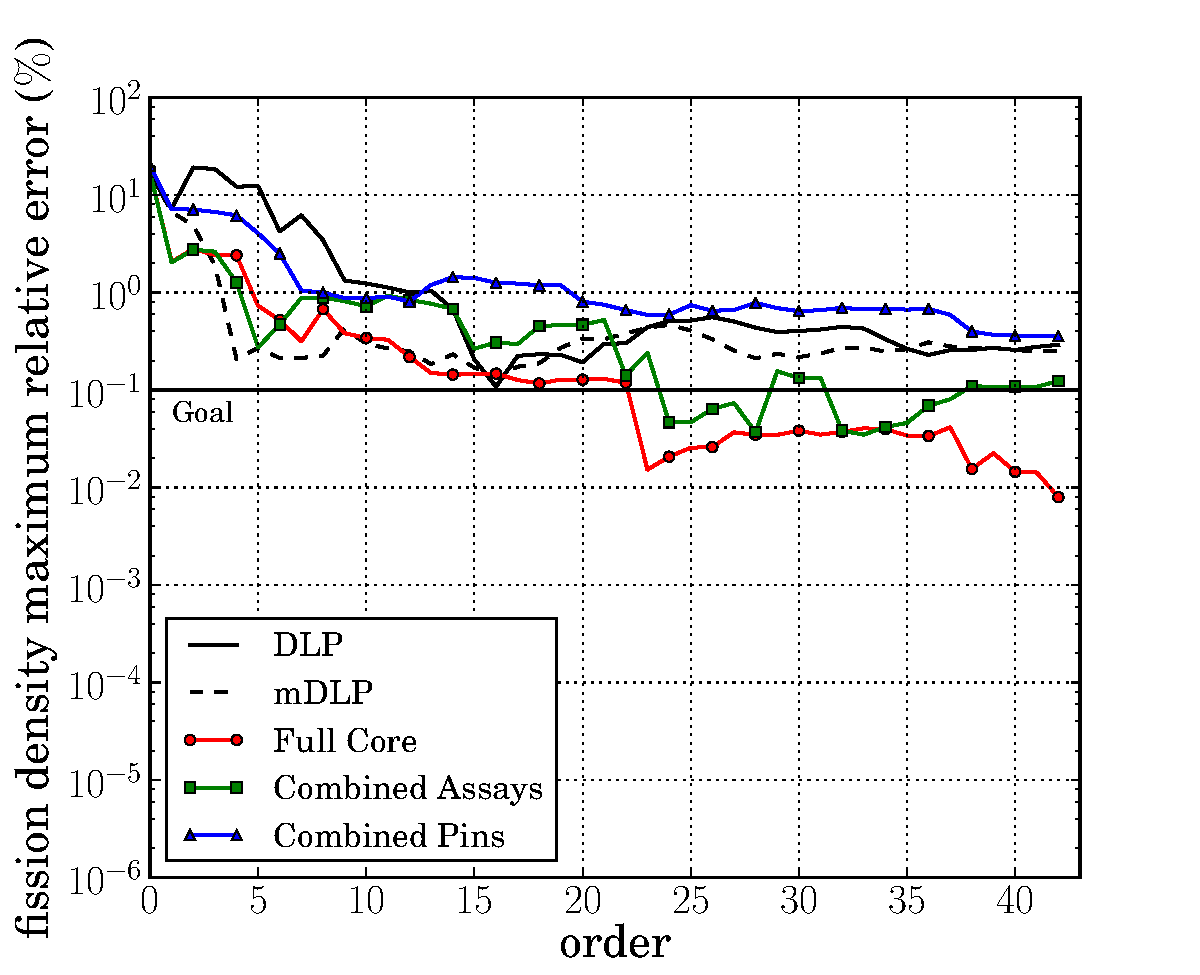
\includegraphics[trim=.1cm .25cm 2.0cm .4cm, clip=true, totalheight=0.28\textheight]{BWR2_238_energy_basis_comparison_fission-44}
      \caption{Using only $\phi$ data}
      \label{fig:core2-238a}
    \end{subfigure}%
    \begin{subfigure}{0.5\textwidth}
      \centering
      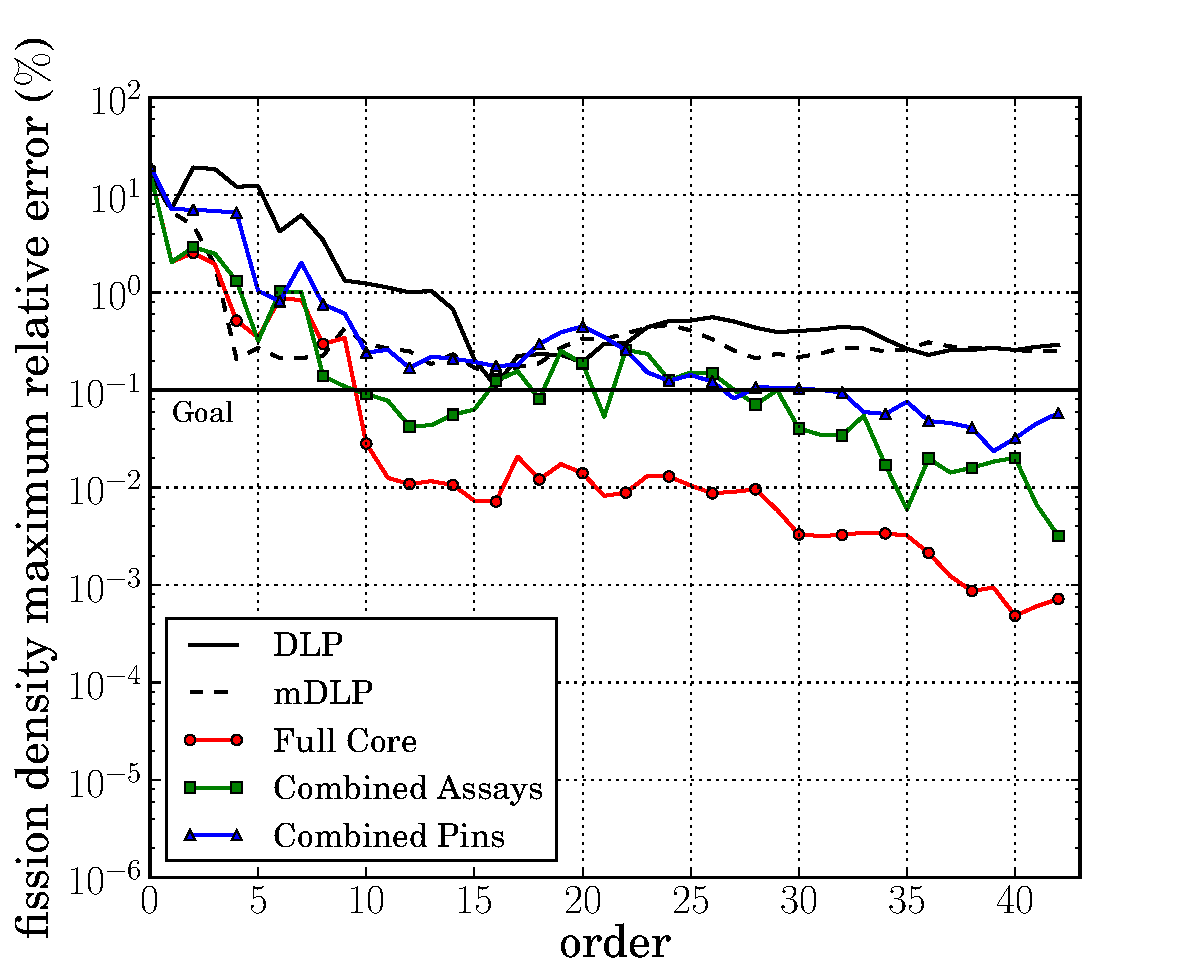
\includegraphics[trim=.1cm .25cm 2.0cm .4cm, clip=true, totalheight=0.28\textheight]{BWR2_238_partial_energy_basis_comparison_fission-44}
      \captionof{figure}{Using $\phi$ and $J_{\text{left}}$ data}
      \label{fig:core2-238b} 
    \end{subfigure}
    \caption{Relative error for BWR test problem, Configuration 2, from 238-group library}
    \label{fig:core2-238}
  \end{figure*}
  
  The realistic models, combined pins and combined assemblies, required energy order of approximately 25 and 15 when using only the 
  scalar flux snapshot and using both scalar flux and partial current, respectively, for Configuration 0.  In Configuration 1,
  the realistic models required at least order 20 to reach the goal when using only scalar flux.  Including partial current
  improved the results to 19th order.  Configuration 2 required at least order 30 when using only scalar flux, but dropped
  to approximately order 25 after including partial current.
  
  Required orders for both test problems was roughly equivalent between the 44-group results and 238-group 
  results, leading to the conclusion that with KLT, the finer details of 238-group data were captured in the low orders, thereby allowing for increased
  order reduction from the 238-group information.  This trend was expected to continue for other test problems that compared number of 
  energy groups.  Once again, the combined pins model performed well in spite of the model simplicity, typically reaching the goal at near the 
  same order as mDLP, despite requiring much less information {\it a priori}.
  
  The higher-order moments were then considered for the BWR test problem.  All three configurations are shown in in Fig. \ref{fig:BWR0_angular}, Fig. \ref{fig:BWR1_angular},
  and Fig. \ref{fig:BWR2_angular}, but the conclusion is identical to the 10-pin case, which is that the higher-order moments did not yield any new information, meaning
  that the relative error derived from higher moments was not significantly different than the $0^{th}$ order moment, which
  was the leftward partial current.
  
  \begin{figure*}[!ht]
    \centering
    \begin{subfigure}{0.5\textwidth}
      \centering
      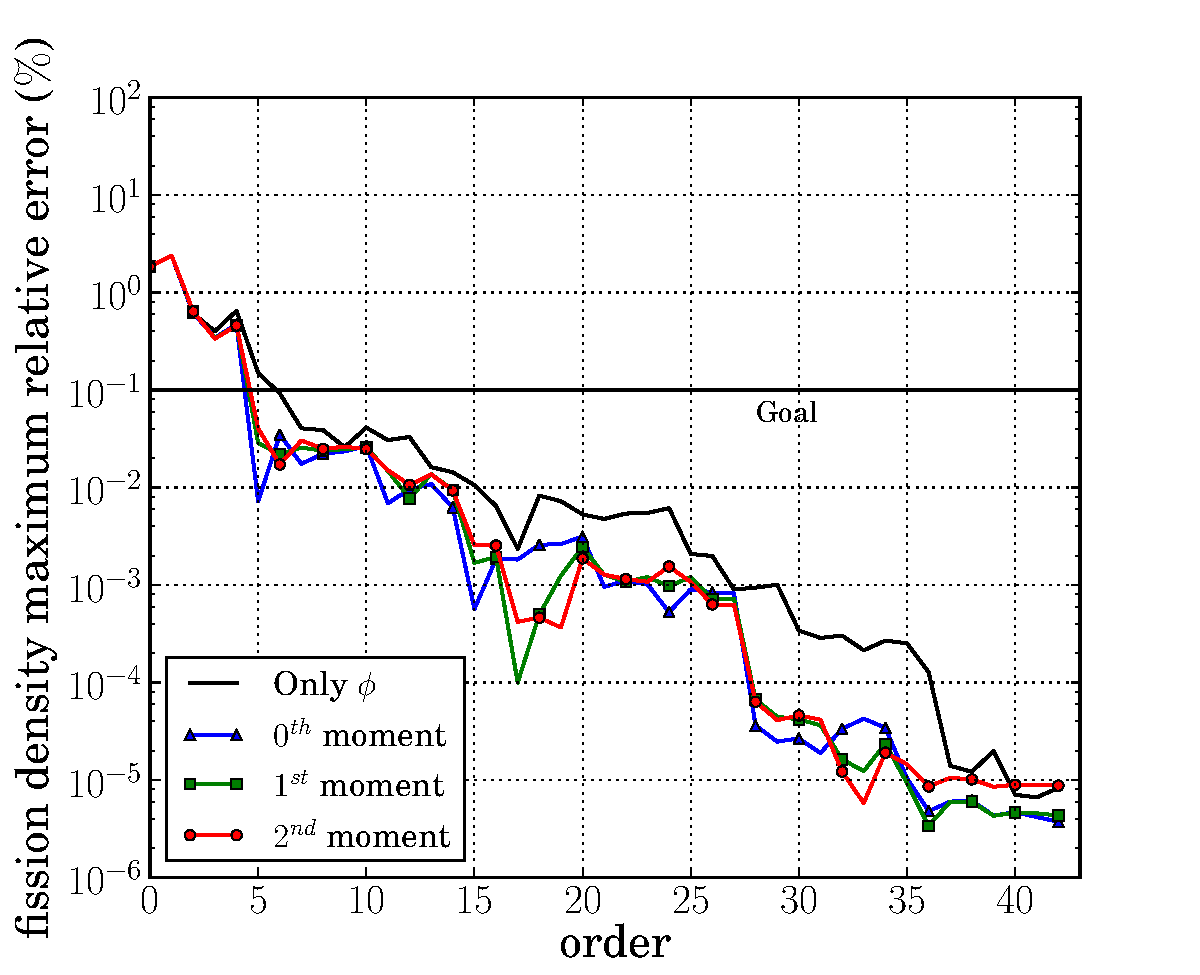
\includegraphics[trim=.1cm .25cm 2.0cm .4cm, clip=true, totalheight=0.28\textheight]{BWR0_44_angular_comparison_fission_core-44}
      \caption{From 44-group library}
      \label{fig:BWR0_angularA}
    \end{subfigure}%
    \begin{subfigure}{0.5\textwidth}
      \centering
      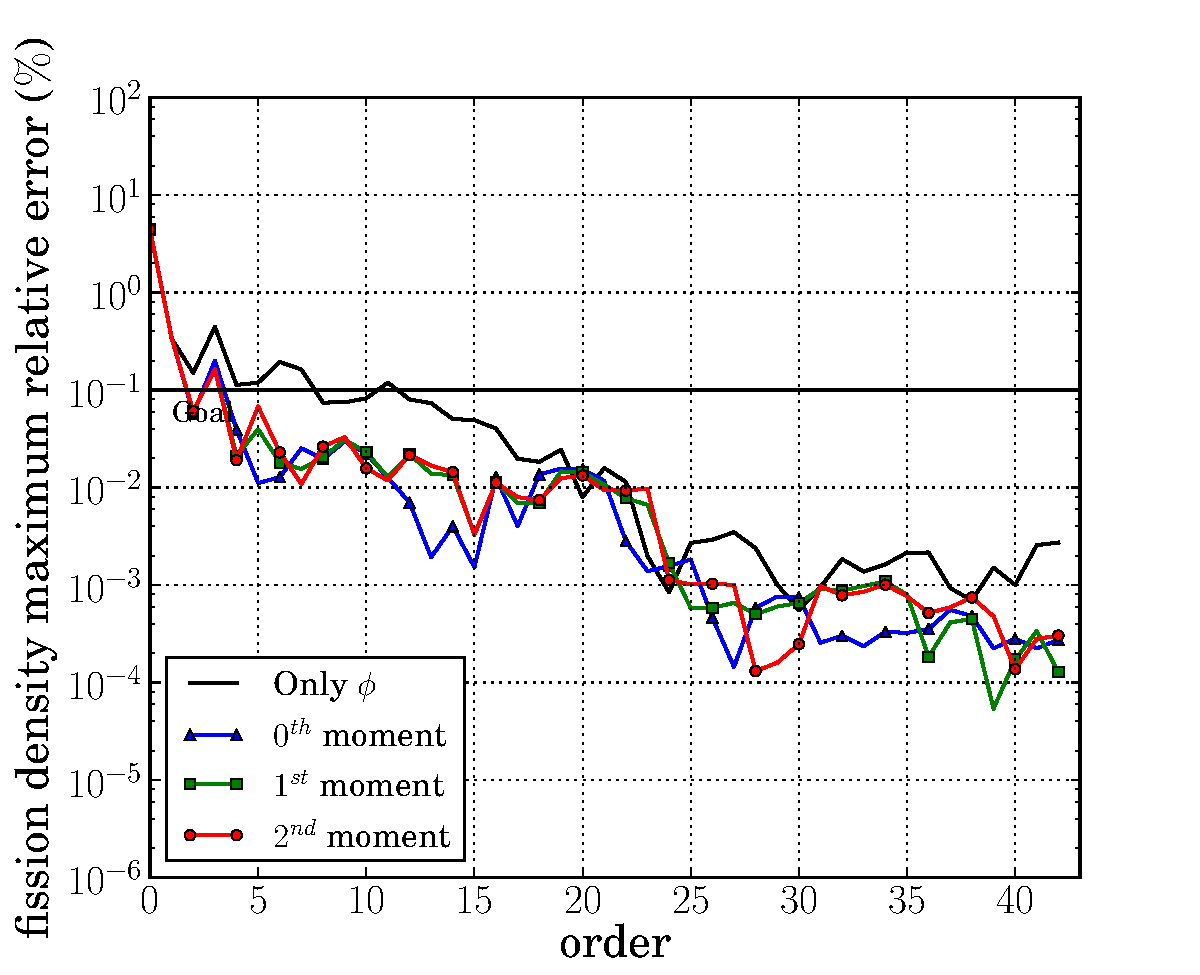
\includegraphics[trim=.1cm .25cm 2.0cm .4cm, clip=true, totalheight=0.28\textheight]{BWR0_238_angular_comparison_fission_core-44}
      \caption{From 238-group library}
      \label{fig:BWR0_angularB}
    \end{subfigure}
    \caption{Relative error for BWR problem, Configuration 0, using higher-order moment data}
    \label{fig:BWR0_angular}
  \end{figure*}
  
  \begin{figure*}[!ht]
    \centering
    \begin{subfigure}{0.5\textwidth}
      \centering
      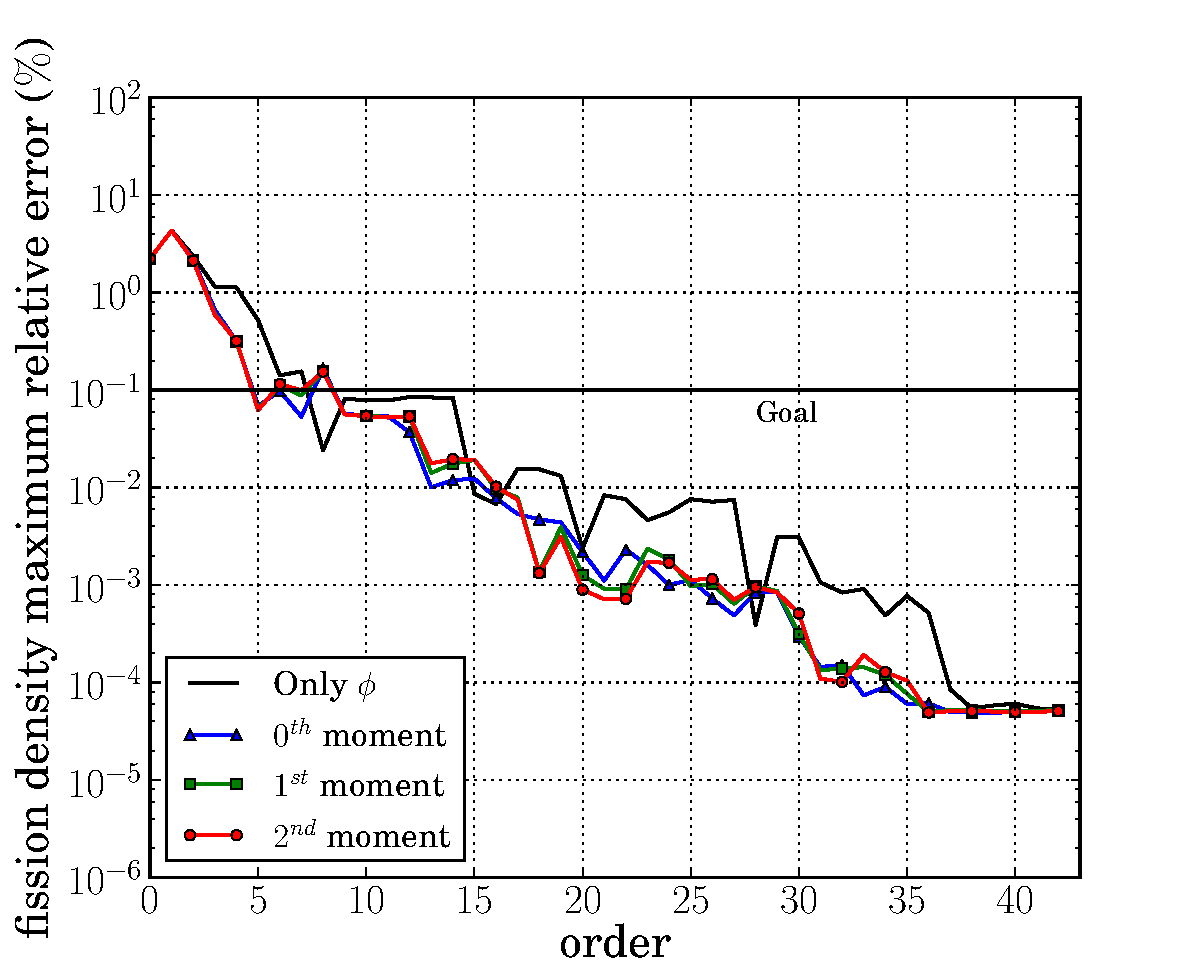
\includegraphics[trim=.1cm .25cm 2.0cm .4cm, clip=true, totalheight=0.28\textheight]{BWR1_44_angular_comparison_fission_core-44}
      \caption{From 44-group library}
      \label{fig:BWR1_angularA}
    \end{subfigure}%
    \begin{subfigure}{0.5\textwidth}
      \centering
      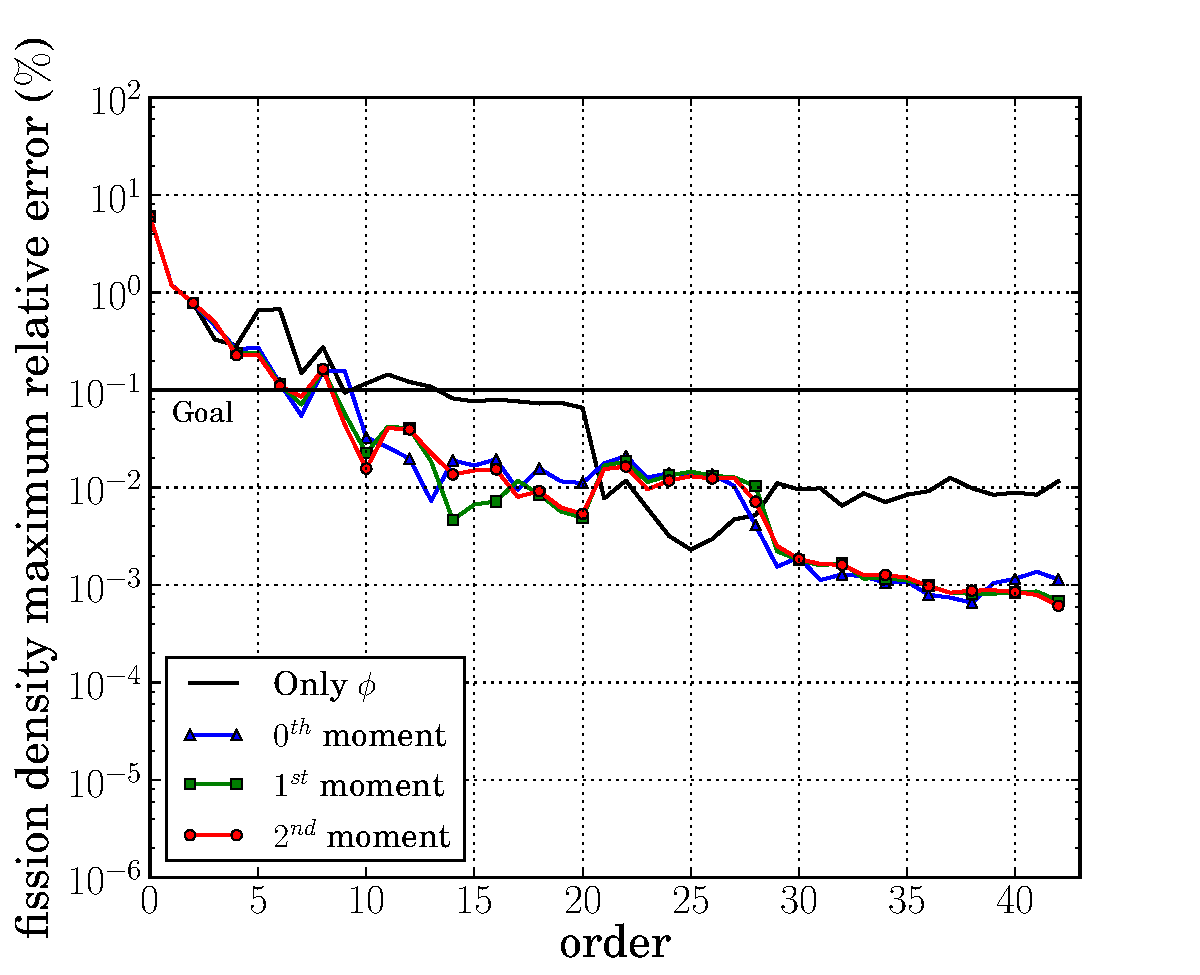
\includegraphics[trim=.1cm .25cm 2.0cm .4cm, clip=true, totalheight=0.28\textheight]{BWR1_238_angular_comparison_fission_core-44}
      \caption{From 238-group library}
      \label{fig:BWR1_angularB}
    \end{subfigure}
    \caption{Relative error for BWR problem, Configuration 1, using higher-order moment data}
    \label{fig:BWR1_angular}
  \end{figure*}
  
  \begin{figure*}[!ht]
    \centering
    \begin{subfigure}{0.5\textwidth}
      \centering
      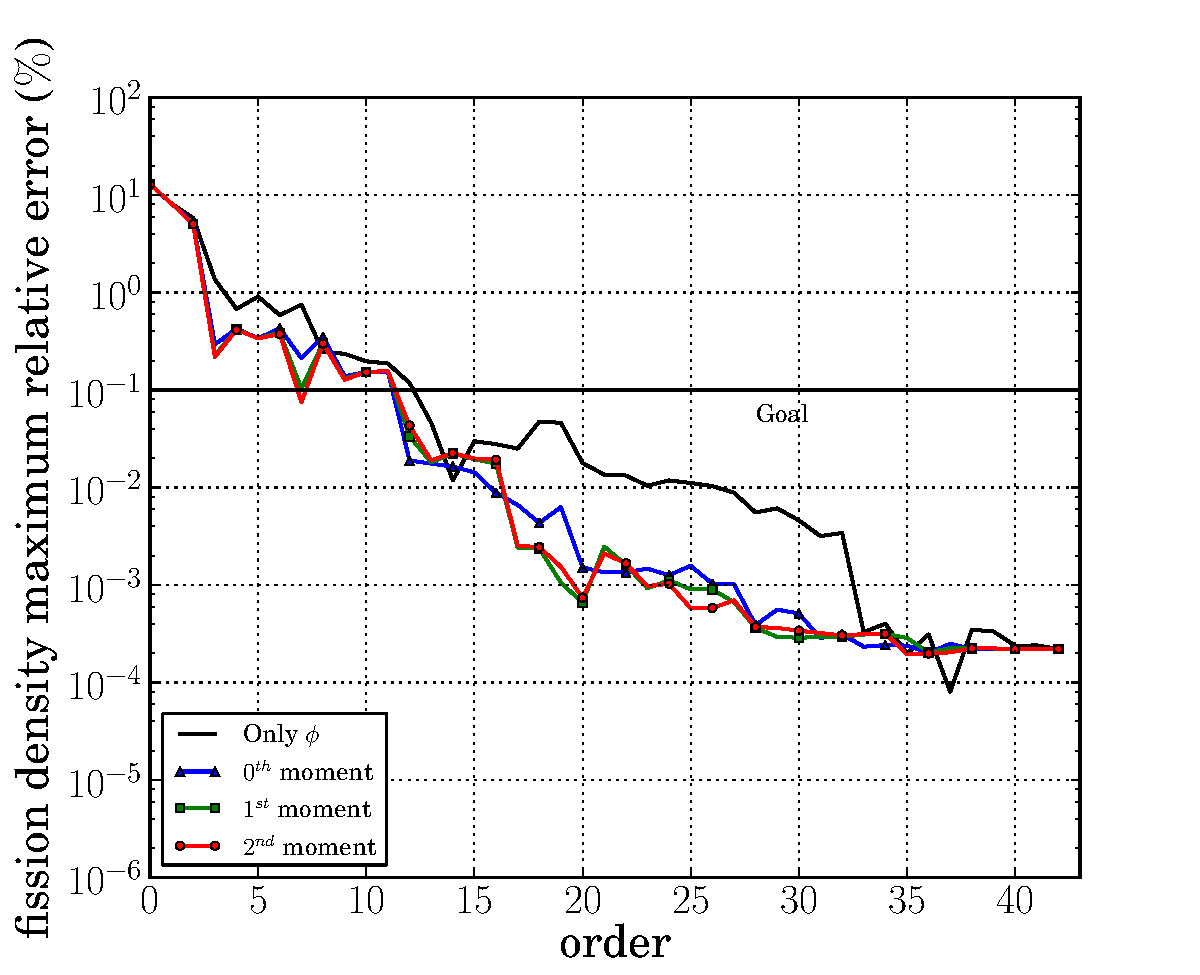
\includegraphics[trim=.1cm .25cm 2.0cm .4cm, clip=true, totalheight=0.28\textheight]{BWR2_44_angular_comparison_fission_core-44}
      \caption{From 44-group library}
      \label{fig:BWR2_angularA}
    \end{subfigure}%
    \begin{subfigure}{0.5\textwidth}
      \centering
      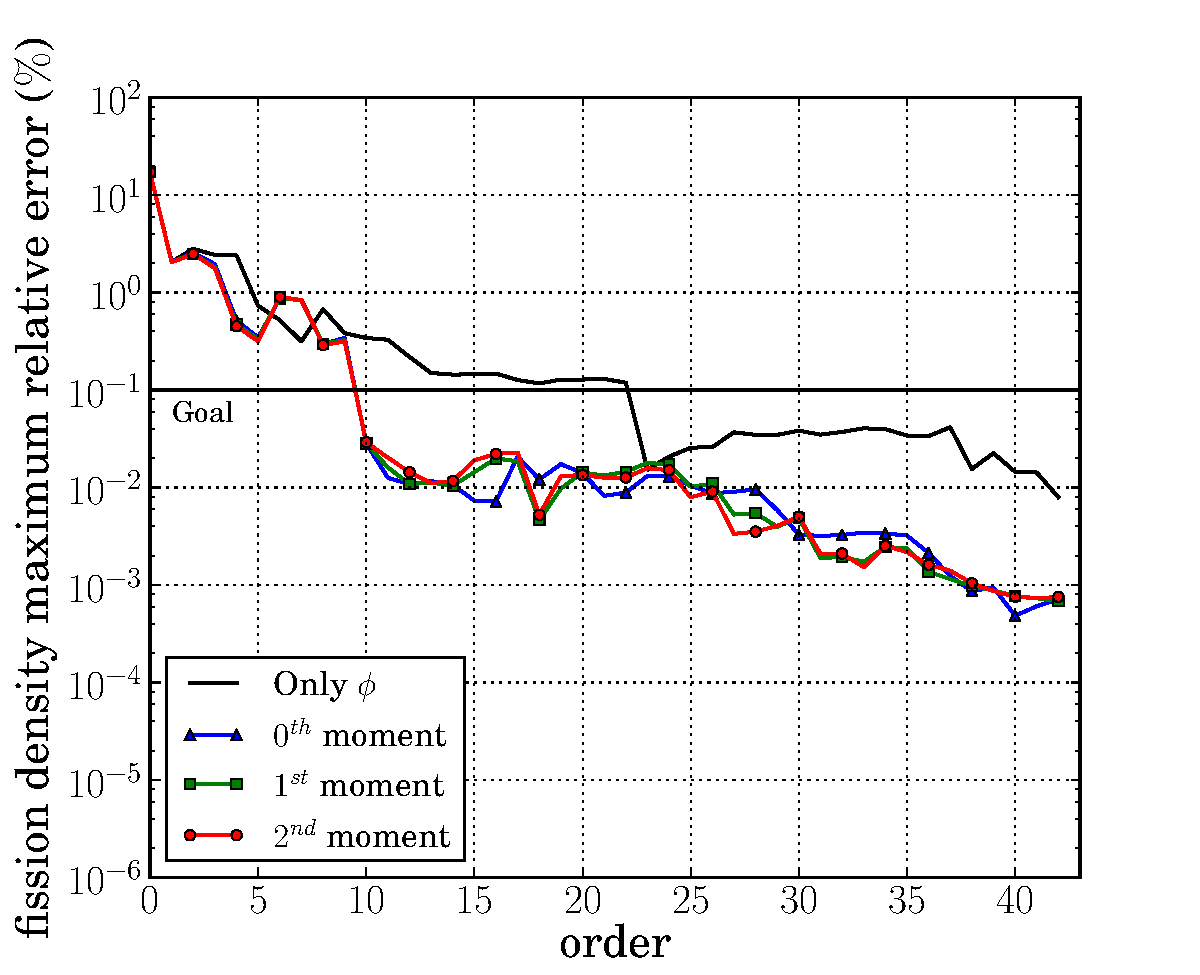
\includegraphics[trim=.1cm .25cm 2.0cm .4cm, clip=true, totalheight=0.28\textheight]{BWR2_238_angular_comparison_fission_core-44}
      \caption{From 238-group library}
      \label{fig:BWR2_angularB}
    \end{subfigure}
    \caption{Relative error for BWR problem, Configuration 2, using higher-order moment data}
    \label{fig:BWR2_angular}
  \end{figure*}
  
  \subsection{Parametric Studies}
  
  To investigate KLT basis sets, several parametric studies were devised and explored.  Two studies that warrant discussion are
  the sensitivity to number of snapshots and to snapshot selection, and the second is the
  sensitivity to selection of snapshots.  For the first study, the 10-pin test problem spatial discretization was varied to produce 
  a greater or smaller number of spatial cells and potential snapshots. Results indicated that mesh size had a relatively 
  small effect on the efficacy of the generated basis set.  Additional snapshots from the same model were exceedingly similar
  to the other snapshots, which did not add additional information to the expansion. 
  
  In the second study, the effect of using a variable number of snapshots from the baseline BWR test problem was studied.  The study 
  used several snapshot selection schemes to select from the total snapshots.  The first scheme was to use evenly spaced snapshots (i.e., only
  every $x$th snapshot was used to generate the basis).  The second used a random selection of a given number.  The third used
  the first $x$ snapshots, and the last scheme used $x$ snapshots from the center (because the problem was spatially symmetric). The
  resulting impact to fission density errors was negligible for the first two schemes, but the last two schemes produced a greater variation until snapshots 
  from all types of cells were included.  In other words, inclusion of additional snapshots did not improve the results unless 
  new snapshots were meaningfully distinct from the current set of snapshots.  Based on these two studies, all available snapshots 
  were used to produce figures in this paper.  The error was not affected by the inclusion of additional, similar snapshots; only 
  computation time was impacted.
  
  \section{Conclusions and Future Work}
  
  KLT basis outperformed the mDLP and DLP bases for ERMM energy expansions because KLT, by construction, maximizes 
  the amount of information contained in low-order expansions. When using appropriate data to generate the basis, sufficient
  accuracy (i.e., sub-$0.1\%$ maximum relative error in fission density) can be obtained with as few as one-tenth of the 
  equivalent energy degrees of freedom used in a full multigroup approximation.  Smaller models used for snapshot generation provided
  encouraging results.  In most cases, the small models were equivalent or outperformed mDLP despite requiring less information {\it a priori}.
  Results were improved by including partial current in snapshot generation.  
  
  When considering test problems using different energy groupings (i.e., 44-group and 238-group), resulting relative 
  fission density errors were approximately the same between the two libraries, suggesting that KLT efficiency is
  almost independent of the number of groups in the library.  Because KLT contains a large amount of physics information in 
  low-order polynomials, KLT can perform as well or better with the inclusion of additional information from the higher
  group library compared to the lower group library.
  
  Results also suggested that adding more snapshots improves the data only if the new snapshots are unique.  Therefore,
  the inclusion of partial current snapshots improved results because the snapshots differed meaningfully from scalar flux snapshots.
  Contrarily, the use of a greater number of snapshots from a finer spatial mesh yielded diminishing improvement because the new 
  snapshots became increasingly similar.  Most problems of interest contain a sufficiently large number of unique spatial
  regions for use in snapshot generation; therefore, a key goal of ongoing work is to determine other variables (e.g, increased angle dependence)
  that can provide greater snapshot variety.  Additional ongoing work aims to extend the use of KLT energy expansions to 2-D problems,
  for which the method is expected to yield similarly encouraging results.
  
  
  %% The Appendices part is started with the command \appendix;
  %% appendix sections are then done as normal sections
  %% \appendix
  
  %% \section{}
  %% \label{}
  
  %% References
  %%
  %% Following citation commands can be used in the body text:
  %% Usage of \cite is as follows:
  %%   \cite{key}         ==>>  [#]
  %%   \cite[chap. 2]{key} ==>> [#, chap. 2]
  %%
  
  %% References with BibTeX database:
  
  \bibliographystyle{elsarticle-num}
  \bibliography{bibliography}
  
  %% Authors are advised to use a BibTeX database file for their reference list.
  %% The provided style file elsarticle-num.bst formats references in the required Procedia style
  
  %% For references without a BibTeX database:
  
  % \begin{thebibliography}{00}
  
  %% \bibitem must have the following form:
  %%   \bibitem{key}...
  %%
  
  % \bibitem{}
  
  % \end{thebibliography}
  
\end{document}

%%
%% End of file `proeng-template.tex'.